% % Second Chapter : Theoritical Approach
%
% Master Thesis: Calibration and Fusion of Stereoscopic and Time-of-Flight 
% Cameras for Zero Gravity Targets Inspection
%
% Achieved at Space System Lab, M.I.T.
% Supervisor: Alvar Saenz-Otero, Daniel Alazard
%
% Institut Sup�rieur de l'A�ronautique et de l'Espace
% Major: Telecommunications et r�seaux - Syst�mes Spatiaux et Lanceurs
% Gabriel Urbain - October 2014
%%

\chapter{Theoretical Approach}
\label{chapter:theory}

In this chapter, we will try to give all the theoretical tools to understand the algorithm development carried out in this project. The first section aims at reminding the reader of background models and theories but we will assume he masters his basics of mechanics of the rigid body, optics, image processing, numerical analysis and computer sciences.
Section two focuses on calibration algorithm. It reviews solutions found in the literature to calibrate separately stereoscopic cameras and a \gls{ToF} camera but also describes the implementation and adaptation of a new algorithm proposed in \cite{stereo_tof_fusion_proba} to calibrate the whole \gls{ToF} and stereo cameras system while taking advantage of each sensors characteristics.
Finally, the last section analyzes the core implementation of the fusion algorithm tested in this project, try to set out arguments to the choices that have been made and describes each parts in details.

\section{Camera Model Elaboration}
Before going into further details into the algorithms breakdown, it may be necessary to clarify the models employed throughout this document. Indeed, to simplify the sensor fusion analysis and implementation, we will have to make numerous simplifications and hypothesis about the camera models that we shall remember in Chapter 4 where experimental results are discussed.

\subsection{Mathematical Notations}
Several coordinates systems are used in this work leading themselves to many different transformations between each others. To give the reader a better overview, this paragraph summarizes the mathematical notations employed in this document.

\paragraph{Coordinates Systems:}
\begin{itemize*}
\item $\mathbf{T}$: Coordinate system of the \gls{ToF}) camera (or \gls{ORF}). In the 3D system, the origin is situated in the pinhole, the  $Z$ axis points forward, $Y$ axis points down and $X$ points right. In the 2D coordinate system, the origin is situated in the top left corner of the image plane,$U$ points to the right and $V$ points down.
\item $\mathbf{R}$: 3D coordinate system of the right camera of the stereo rig. In the 3D system, the origin is situated in the pinhole, the  $Z$ axis points forward, $Y$ axis points down and $X$ points right. In the 2D coordinate system, the origin is situated in the top left corner of the image plane,$U$ points to the right and $V$ points down.
\item $\mathbf{L}$: 3D coordinate system of the left camera of the stereo rig. In the 3D system, the origin is situated in the pinhole, the  $Z$ axis points forward, $Y$ axis points down and $X$ points right. In the 2D coordinate system, the origin is situated in the top left corner of the image plane,$U$ points to the right and $V$ points down.
\end{itemize*}

\paragraph{Transformations Matrices:}
To represent both affine (translation and rotation) and projective transformation  from one coordinate system to another, we use $4x4$ transformation matrices. For instance, in the case of an affine transformation of a point $P$ from $R$ to $L$ coordinate system, we write:
\begin{equation}
\begin{pmatrix}[0.8]
x_L\\
y_L\\
z_L\\
1
\end{pmatrix} = M_{LR} * \begin{pmatrix}[0.8]
x_R\\
y_R\\
z_R\\
1
\end{pmatrix}
\end{equation}
Where:
\begin{equation}
M_{LR} = \begin{pmatrix}[0.8]
r_{XX} & r_{XY} & r_{XZ} & t_X\\
r_{YX} & r_{YY} & r_{YZ} & t_Y\\
r_{ZX} & r_{ZY} & r_{ZZ} & t_Z
\end{pmatrix}
\end{equation}
Which allows to multiply matrices directly between each other:
\begin{equation}
M_{TR} = M_{TL} * M_{LR}
\end{equation}


\subsection{Pinhole Camera Model}
\label{sec:mono_camera}
According to \cite{epipolar_geometry}, a common representation of a camera is composed of a lens represented by a single pinhole $O$ in the \textit{focal plane }$\mathcal{F}$ and a sensor matrix in the \textit{image plane} $\mathcal{I}$ at a distance $f$ from the focal plane. As represented on figure \ref{fig:cam1}, $O$, also called optical center, is the origin of the world 3D coordinates system $OXYZ$ where $Z$ is perpendicular to the focal plane and directed in the opposite direction of the image plane and $X$ and $Y$ are included in the plane. The pixels on the image plane are localized with a 2D coordinates system $O'U'V'$ where the origin is situated in the lower-right corner of the sensor matrix. The $Z$ axis intersects $\mathcal{I}$ in a point $c' = (c_U', c_V')$ called the \textit{principal point}.

% Figure cam1
\begin{figure}[!htt]
	\begin{center}
		\includegraphics[width=15cm]{img/cam1.png}
		\caption{Geometry of the pinhole model for a single camera}
		\label{fig:cam1}
	\end{center}
\end{figure}

To facilitate the representation, we can consider a \textit{virtual image plane} at a distance $f$ on the positive $Z$ axis, which does not change anything to the problem but helps to recreate directly a \textit{projected image} with the same orientation than the real object. We now have a 2D coordinate system $O"UV$ (figure \ref{fig:cam2}).

% Figure cam2
\begin{figure}[!htt]
	\begin{center}
		\includegraphics[width=15cm]{img/cam2.png}
		\caption{In this simplified representation, the point P is projected in the virtual plane}
		\label{fig:cam2}
	\end{center}
\end{figure}

In this optimal model, the \textit{intrinsic} geometry of the camera is completely represented by the parameters $f$, $c_U$ and $c_V$ measured in pixels. However, to make the model more realistic, we can introduce extra parameters such as:
\begin{itemize*}
\item The lens enlargement $k$, whose value is different along $u$ and $v$ axis and represented in the model by coordinates $f_U = k_U * f$ and $f_V = k_V * f$
\item The skew $s_{UV}$, assessing the non-orthogonality between rows and columns of the sensor photosensitive cells.
\end{itemize*}
Those five parameters $f_U$, $f_V$, $c_U$, $c_V$, $s_{UV}$ constitute what we call the \textit{intrinsic matrix} of the camera:
\begin{equation}
K =  \begin{pmatrix}
	f_U & s_{UV} & c_U\\
	0 & f_V & c_V\\
	0 & 0 & 1
	\end{pmatrix}
\end{equation}

Therefore, we can write the affine transformation linking a \textit{world point}, represented by its \textit{homogeneous coordinates} in the camera three-dimensional coordinates system and a \textit{projected point} represented by its \textit{homogeneous coordinates} in the image two-dimensional coordinates system:
\begin{equation}
\label{eq:pinhole}
s \begin{pmatrix}[0.8]
u\\
v\\
1
\end{pmatrix}
 = K * \begin{pmatrix}[0.8]
 x\\
 y\\
 z\\
 1
 	\end{pmatrix}
\end{equation}

Finally, the model can be refine to take the distortions into account. As proposed by Brown \cite{camera_distortion}, the distortion may be divided into radial and tangential and can be represented by a second degree polynomial which maps the undistorted and distorted images together thanks to 6 parameters. This will be detailed in section \ref{sec:calib}.\\

One should also notice that the parameters discussed here define the mathematical model of the camera but performances can be determined as well. For instance, the \textit{Field-Of-View} (\gls{FoV}) of the camera and the pixel size $\epsilon_p$ of the photosensitive cells (sometimes given by the pixel density, measured in pix/meters) are two characteristics to measure camera performances.

\subsection{Stereoscopic Cameras Model}
\label{sec:stereo_camera}
In the literature, the stereo camera is commonly represented as the assembly of two pinhole models whose focal points are separated by a distance called \textit{baseline}. As in figure \ref{fig:cam_stereo}, we thus have now two 3D coordinate systems $L = O_LX_LY_LZ_L$ and $R = O_RX_RY_RZ_R$.

% Figure cam_stereo
\begin{figure}[!htt]
	\begin{center}
		\includegraphics[width=15cm]{img/cam_stereo.png}
		\caption{Model of an assembly of stereoscopic cameras}
		\label{fig:cam_stereo}
	\end{center}
\end{figure}

\subsubsection{Projection}
We can still use the model developed in the precedent paragraph but the rotation and the translation between $L$ and $R$ must be taken into account when a point is represented in 3D. An \textit{extrincic matrix} is then defined to perform that transformation:
\begin{equation}
M =  \begin{pmatrix}
	r_{X,X'} & r_{X,Y'} & r_{X,Z'} & t_{X}\\
	r_{Y,X'} & r_{Y,Y'} & r_{Y,Z'} & t_{Y}\\
	r_{Z,X'} & r_{Z,Y'} & r_{Z,Z'} & t_{Z}
	\end{pmatrix}
\end{equation}

Which gives:
\begin{equation}
s \begin{pmatrix}
u\\
v\\
1
\end{pmatrix}
 = K * M * \begin{pmatrix}[0.8]
 x\\
 y\\
 z\\
 1
 	\end{pmatrix} = P * \begin{pmatrix}[0.8]
 	 x\\
 	 y\\
 	 z\\
 	 1
 	 	\end{pmatrix}
\end{equation}

Where $P$ is also called the \textit{projection matrix}.

When we write the equations for both left and right cameras, the \textit{extrinsic matrix} can either refer to a third coordinate system, either to $L$ or $R$. In the last case, one of the two $M$ matrix is useless. For instance, if we consider the world coordinate system as $L$, we now write:
\begin{equation}
\label{eq:stereo}
\begin{cases}
s \begin{pmatrix}[0.8]
	u_L\\
	v_L\\
	1
	\end{pmatrix}
= K_L * \begin{pmatrix}[0.8]
	x\\
	y\\
	z\\
	1
	\end{pmatrix}\\
s \begin{pmatrix}[0.8]
	u_R\\
	v_R\\
	1
	\end{pmatrix}
= K_R * M_R * \begin{pmatrix}[0.8]
	x\\
	y\\
	z\\
	1
	\end{pmatrix}
\end{cases}
\end{equation}

As for the camera model, those equations can be used to compute directly $(u_L, v_L)$ and $(u_R,v_R)$ from the 3D coordinates of a point with the knowledge of \textit{intrinsic} and \textit{extrinsic} matrices for both cameras. This process is known as \textit{\textbf{projection}}.

\subsubsection{Triangulation}
Intuitively, if inverting the pinhole equation was not directly useful with a mono camera because there was one degree of freedom remaining, we can invert the stereo cameras model to find the 3D coordinates from the projected points in $L$ and $R$. However, this process, known as \textit{\textbf{triangulation}}, requires the triangulated points to respect the \textit{epipolar constraint} in order to give coherent results \cite{multiple_view}, i.e. $(u_L,v_L)$ and $(u_R, v_R)$ must be defined to ensure that the two \textit{epipolar rays} from $L$ and $R$ cross in one point in the real world as represented in figure \ref{fig:cam_stereo}.

Practically, in the 3D reconstruction from stereo sensors problem, the points $p_L = (u_L, v_L)$ and $p_R = (u_R, v_R)$ in the focal images are found using image processing techniques, as developed in \ref{subsec:fusion:overview}. The precision of this method, the accuracy of the physical sensors, the precision of the calibration matrices, the numerical errors,... Everything makes this constraint difficult to respect. We can therefore consider two ways to overcome this issue:
\paragraph{Simplify the problem}: In the first option, we suppose the cameras to be perfectly aligned in $Y$ and $Z$ coordinates, the \textit{baseline} is measured on the $X$ axis. Thus, \textit{epipolar lines} are totally included in $XZ$ planes for each points and as soon as those one are visible in left and right images, they will cross for sure. This leads to simplified projection matrices:
\begin{equation}
P_L = \begin{pmatrix}
	f & 0 & c_U & 0\\
	0 & f & c_V & 0\\
	0 & 0 & 1 & 0
	\end{pmatrix}
\end{equation}
\begin{equation}
P_R = \begin{pmatrix}
	f & 0 & c_U & t_{LR}\\
	0 & f & c_V & 0\\
	0 & 0 & 1 & 0
	\end{pmatrix}
\end{equation}

\paragraph{Minimize errors}: The other solution is to keep an elaborate model where left and right cameras can be misaligned but try to minimize the sum of euclidean errors when we are triangulating many points. Various algorithm concerning the subject have been analyzed in \cite{multiple_view} or \cite{triangulation}.

The two kinds of \textit{triangulation} and \textit{projection} methods have been implemented in the stereo cameras software but this thesis mostly focus on the first one for it is easier to implement and give sufficient results with \gls{VERTIGO} \cite{muggler_phd}.

\subsection{Optical Range Finder Model}
\label{sec:ORF_model}
A Time-Of-Flight camera (\gls{ToF}), also called Optical Range Finder (\gls{ORF}) in this document, is a class of LIDAR that can measure an entire 3D scene in real-time (more than 25 FPS) \cite{TOF_principle}\cite{TOF}. As shown in figure \ref{fig:cam_orf} modulated light bursts illuminating the scene are produced by an IR emitter on the camera, the light is scattered by objects in the scene and a fast CMOS sensor synchronized with the emitter samples the received pulse and retrieves its phase. For each pixel, a distance camera-object can be compute as:
\begin{equation}
d = \dfrac{c}{2}.\dfrac{\Delta\phi}{2 \pi f}
\end{equation}
Where:
\begin{itemize*}
\item $\Delta \phi$ is the phase shift between the emitted and received light
\item $c$ is the light speed: $299 792 458 m/s$
\item $f$ is the IR modulation frequency which has been set to $15MHz$ in our experiments
\end{itemize*}
Which also means that the camera maximal range $D$ is equal to $10m$.

% Figure cam_orf
\begin{figure}[!htt]
	\begin{center}
		\includegraphics[width=14cm]{img/cam_orf.png}
		\caption{Principle of a time-of-flight camera. The pinhole model is still applicable for the geometry but the measurement of the phase allows to create a new image: the \textit{depth map} $D_T$}
		\label{fig:cam_orf}
	\end{center}
\end{figure}

In addition to the \textit{depth map} $D_T$, two other images can be extracted from the sensor. In figure \ref{fig:cam_orf_2} provided by the Data Sheet of the camera, we are using \cite{SR4k_manual}, $A$ is a measure of the modulated signal amplitude and helps to compute a \textit{confidence map} $C_T$ (the larger $A$, the better confidence on the measure); $B$ is a measure of the mean signal amplitude and gives a \textit{visual image} $V_T$ very similar to the one we can have with traditional black and white cameras.

% Figure cam_orf_2
\begin{figure}[!htt]
	\begin{center}
		\includegraphics[width=12cm]{img/cam_orf_2.png}
		\caption{The received modulated IR signal is sampled and three images can be computed from the parameters $A$, $B$ and $\Delta \phi$: \textit{depth map} $D_T$, \textit{confidence map} $C_T$ and \textit{visual image} $V_T$ - \textit{Mesa Imaging SR4k Data Sheet \cite{SR4k_manual}}}
		\label{fig:cam_orf_2}
	\end{center}
\end{figure}




\section{Calibration Algorithm}
\label{sec:calib}
\subsection{Literature Overview}
The calibration is a process that aims at finding the most accurate \textit{instrinsic} and \textit{extrinsic} matrices of the pinhole model described in sections \ref{sec:mono_camera} and \ref{sec:stereo_camera} without any prior knowledge of the camera geometry. A precise camera calibration constitutes an important problem since it determines the accuracy of the results. Thus, numerous alternate methods have been developed to guarantee the best possible calibration. According to \cite{intrinsic_calib}, this process can be divided into three categories:
\begin{itemize*}
\item \textbf{3D object-based calibration}: The known geometry of a 3D object as well as its projection are used to compute the best matrices that verify the pinhole equation \ref{eq:pinhole}. It however requires the presence of an accurate 3D calibration target for each calibration.
\item \textbf{Self-calibration}: No object is used but the rigidity of a static environment induces enough constraints to estimate the calibration parameters. If this is very flexible, it is still not always reliable as a lot of initial parameters has to be estimated.
\item \textbf{2D pattern-based calibration}: This third category is a compromise of flexibility (it requires only a 2D pattern like a checkerboard) and reliability (the solution always converges).
\end{itemize*}
\subsubsection{\gls{ORF} calibration}
Calibrating the \gls{ORF} can be seen as a single camera calibration as it involves only the estimation of the \textit{intrinsic matrix}. Different methods has been proposed in \cite{tof_calibration} or \cite{tof_calibration_2}. Due to its success, the Brown method presented in \cite{intrinsic_calib} and \cite{intrinsic_calib_1} will be considered. 
Apart from the \textit{intrinsic} calibration, we shall however notice that \cite{stereo_tof_fusion_proba} and \cite{tof_calibration_1} explain that we shall correct the systematic depth measurement error and this can be realized with a polynomial correction functional approach.
\subsubsection{Stereoscopic cameras calibration}
This category is relatively old, which is an advantage since we can find numerous efficient ways to realize them in the literature. For example, in the \gls{VERTIGO} project, the Brown method \cite{camera_distortion} has been tested through the \textit{OpenCV} libraries \cite{opencv} leading to satisfying results \cite{vertigo_phd}.
\subsubsection{\gls{ORF}-stereo system calibration}
This last category aims at finding \textit{extrinsic matrices} between the \gls{ORF} camera and the stereo cameras assembly. Since the problem is quite recent, different algorithms have been proposed these last few years in \cite{stereo_tof_fusion_proba}, \cite{stereo_tof_fusion_accuracy}, \cite{tof_calibration_1}. In this paper, we will focus on the algorithm presented in \cite{stereo_tof_fusion_proba} because besides the \gls{ORF} \textit{visual image} whose space resolution is very low, the process also takes profit of the \textit{depth map} to increase the accuracy.


\subsection{Optical Range Finder Calibration}
As the \gls{ORF} can be seen as a simple camera, the goal of the process is to find the matrix $K$ in the pinhole equation:
\begin{equation}
s \begin{pmatrix}[0.8]
u_T\\
v_T\\
1
\end{pmatrix}
 = K * \begin{pmatrix}[0.8]
 x_T\\
 y_T\\
 z_T\\
 1
 	\end{pmatrix}
\end{equation}
Let's take a set of world points $P_T^i$ ($i=1...m$) and their projection $p_T^i$. For each $i$, this equation ca be rewritten:
\begin{equation}
\label{eq:K}
p_T^i = \begin{pmatrix}[0.8]
u\\
v
\end{pmatrix}_T^i =  \mathcal{K}(f_U, f_V, c_U, c_V, s_{UV}, P_T^i)
\end{equation}
If we consider now the distortion model proposed in \cite{camera_distortion}, we can match initial coordinates $(u_{init},v_{init})$ in the \textit{image plan} with \textit{undistorted} coordinates $(u_{corr}, v_{corr})$ in the same plan through the equation:
\begin{equation}
\label{eq:D}
p_{corr}^i = \begin{pmatrix}[0.8]
u\\
v
\end{pmatrix}_{corr}^i =  \mathcal{D}(u_{init}^i, v_{init}^i, k_1, k_2, k_3, k_4, k_5)
\end{equation}
Where:
\begin{equation}
	\begin{cases}
		u_{corr} = u * (1 + k_1 r + k_2 r^4 + k_3 r^6) + 2 k_4 u v_ + k_5 (r^2 + 2 u^2)\\
		v_{corr} = v * (1 + k_1 r + k_2 r^4 + k_3 r^6) + k_4 (r^2 + 2 v^2) + 2 k_5 u v\\
		r = \sqrt{u + v}\\
		u = \dfrac{u_{init}}{z}\\
		v = \dfrac{v_{init}}{z}\\
	\end{cases}
\end{equation}
From \ref{eq:K} and \ref{eq:D}, we can write then:
\begin{equation}
\label{eq:F}
p_T^i = \begin{pmatrix}[0.8]
u\\
v
\end{pmatrix}_T^i =  \mathcal{F}(f_U, f_V, c_U, c_V, s_{UV}, k_1, k_2, k_3, k_4, k_5, P_T^i)
\end{equation}
Or more simply:
\begin{equation}
\label{eq:F2}
p_T^i =  \mathcal{F}(\theta_T^i)
\end{equation}
If we define $\theta_T^i = (f_U, f_V, c_U, c_V, s_{UV}, k_1, k_2, k_3, k_4, k_5, P_T^i)$ as the unknown vector.

Practically, all those points $P_T^i$ correspond to the points on a plane pattern (the corner of a checkerboard). Therefore, to find the vector $\theta_T^i$, we detect the checkerboard corners projections $p_T^i$ in the \textit{visual image} $V_T$, we create an initial guess $\hat{\theta}_T^i$ for each point and we solve the constrained iterative least square problem:
\begin{equation}
\label{eq:calib_min}
\theta_T^i = \mathtt{arg}\enspace \mathsf{min}\,\bigg\{\sum_{i=1}^m\, \lVert\mathcal{F}(\hat{\theta}_T^i) - p_T^i\rVert^2\bigg\}
\end{equation}
Where constraints are:
\begin{itemize*}
\item \textit{All points are in the same plane}
\item \textit{The distance between two consecutive points is known}
\end{itemize*}
As the iterative algorithm used to solve the problem \ref{eq:calib_min} has been detailed in \cite{intrinsic_calib} and already implemented in OpenCV, we will not go into further details but understanding how the problem is defined will be useful in the following sections.


\subsection{Stereoscopic Cameras Calibration}
In a stereoscopic calibration, the same thought process can be applied as in the previous paragraph except that \textit{intrinsic} and \textit{extrinsic} matrices for both cameras must be estimated in the same time. Indeed, we start from the equation system \ref{eq:stereo}, which gives after rewriting:
\begin{equation}
\label{eq:F_stero}
\begin{pmatrix}[0.8]
	p_L\\
	p_R
\end{pmatrix}^i
=  \mathcal{F}_{stereo}(\theta_{stereo})
\end{equation}
Where:
\begin{equation}
\theta_{stereo} = \begin{pmatrix}[0.8]
f_U^L, f_V^L, c_U^L, c_V^L, s_{UV}^L, k_1^L, k_2^L, k_3^L, k_4^L, k_5^L, P_L^i\\
f_U^R, f_V^R, c_U^R, c_V^R, s_{UV}^R, k_1^R, k_2^R, k_3^R, k_4^R, k_5^R, P_R^i\\
M_LR
\end{pmatrix}
\end{equation}
The minimization problem is then:
\begin{equation}
\label{eq:calib_min_stereo}
\theta_{stereo}^i = \mathtt{arg}\enspace \mathsf{min}\,\bigg\{\sum_{i=1}^m\, \bigg\lVert\mathcal{F}_{stereo}(\hat{\theta}_{stereo}^i)
- \begin{pmatrix}[0.8]
p_L\\
p_R
\end{pmatrix}^i\bigg\rVert^2\bigg\}
\end{equation}
The constraints are now:
\begin{itemize*}
\item \textit{All points are in the same plane}
\item \textit{The distance between two consecutive points is known}
\item \textit{Two epipolar lines cross in one single point (or the error is minimized in the case of a complex model)}
\end{itemize*}

\subsection{Multi-Sensors Calibration}
\label{subsec:system_calib}
In this third and last part of calibration, we focused on the estimation of the extrinsic matrix between the \gls{ORF} and the stereoscopic cameras. As  explained in the literature review, this method proposed in \cite{stereo_tof_fusion_proba} takes advantage of all the information given by the sensors and not only of visual images. Figure \ref{fig:calib_arch} shows the architecture of this method and theoretical details are given in the following paragraphs.

% Figure calib_arch
\begin{figure}[!htt] 
	\begin{center}
		{\scalefont{0.5}
		% Graphic for TeX using PGF
% Title: /home/gabs48/mit/thesis/graphic/calib_arch.dia
% Creator: Dia v0.97.2
% CreationDate: Fri Oct 10 14:03:20 2014
% For: gabs48
% \usepackage{tikz}
% The following commands are not supported in PSTricks at present
% We define them conditionally, so when they are implemented,
% this pgf file will use them.
\ifx\du\undefined
  \newlength{\du}
\fi
\setlength{\du}{15\unitlength}
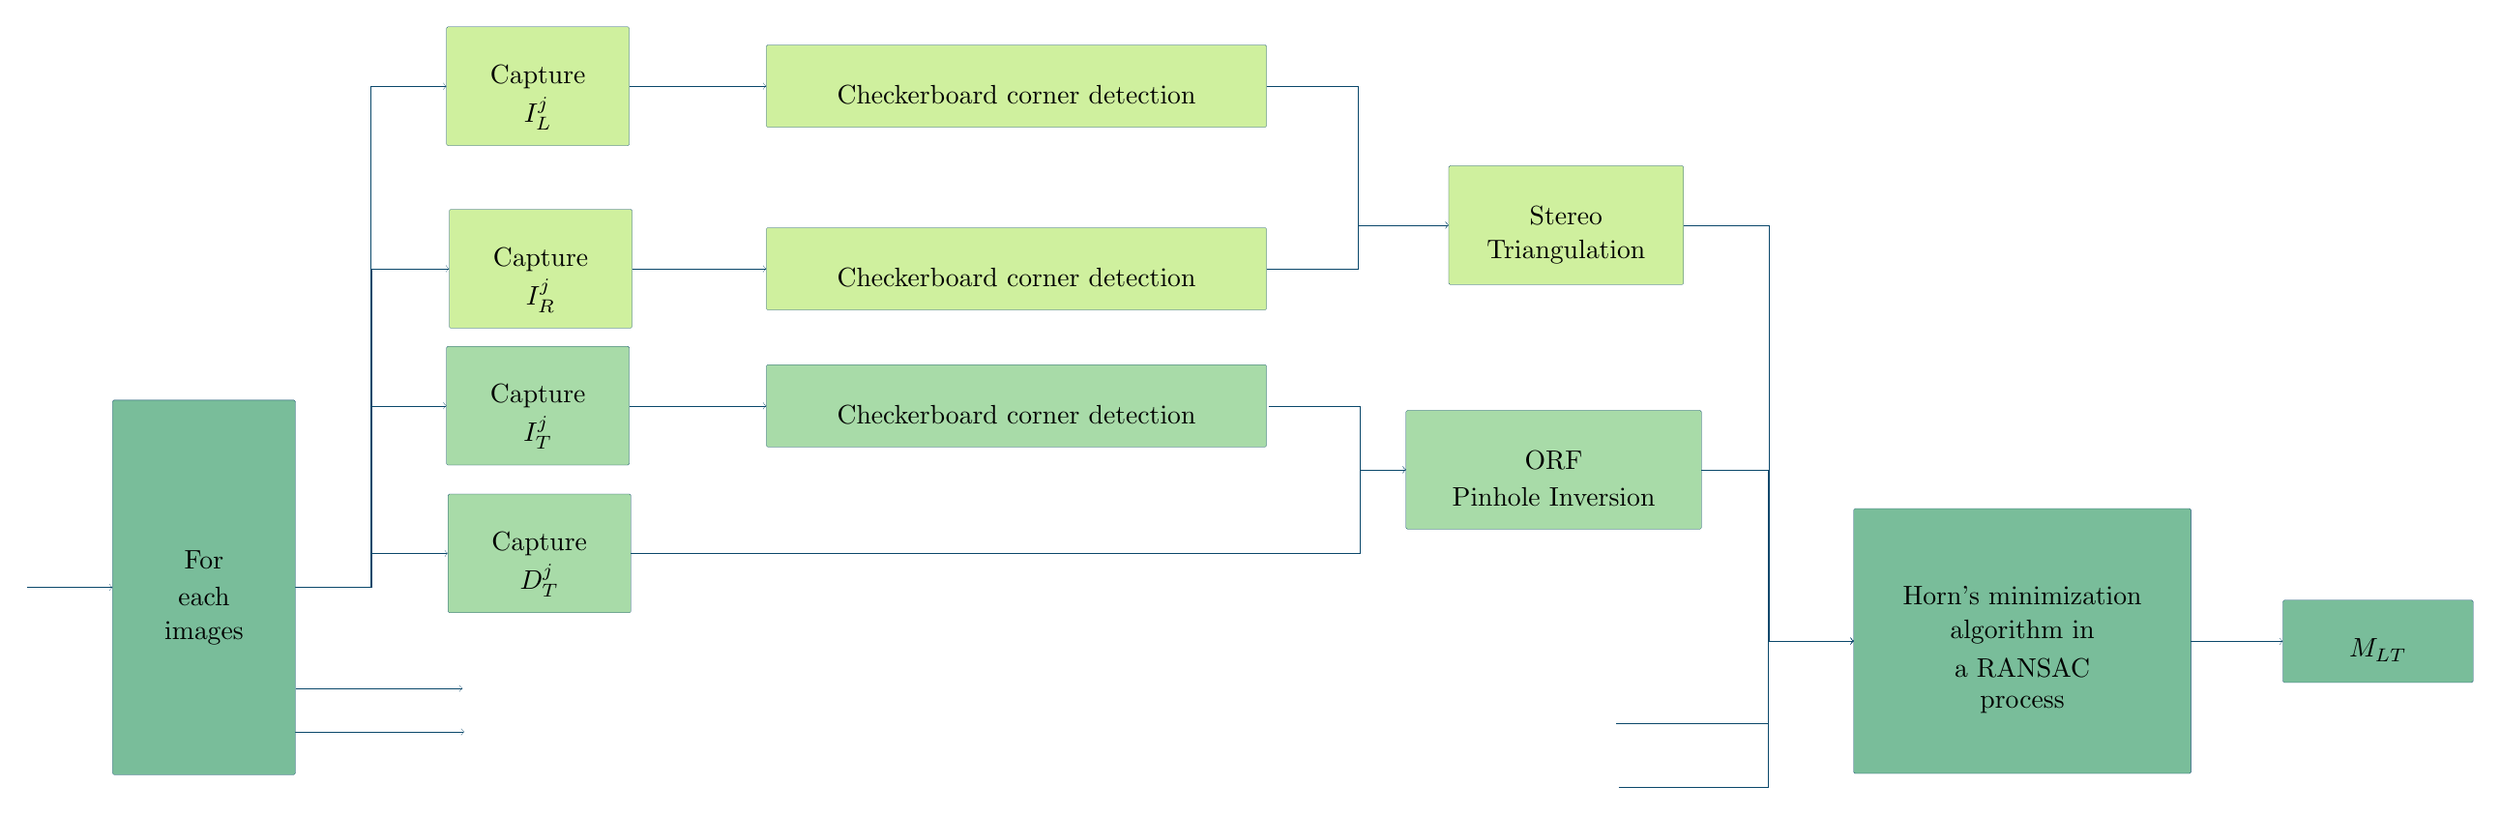
\begin{tikzpicture}
\pgftransformxscale{0.600000}
\pgftransformyscale{-0.600000}
\definecolor{dialinecolor}{rgb}{0.000000, 0.000000, 0.000000}
\pgfsetstrokecolor{dialinecolor}
\definecolor{dialinecolor}{rgb}{1.000000, 1.000000, 1.000000}
\pgfsetfillcolor{dialinecolor}
\pgfsetlinewidth{0.100000\du}
\pgfsetdash{}{0pt}
{\pgfsetcornersarced{\pgfpoint{0.500000\du}{0.500000\du}}\definecolor{dialinecolor}{rgb}{0.811765, 0.941176, 0.619608}
\pgfsetfillcolor{dialinecolor}
\fill (15.000000\du,11.000000\du)--(15.000000\du,12.800000\du)--(25.947500\du,12.800000\du)--(25.947500\du,11.000000\du)--cycle;
}{\pgfsetcornersarced{\pgfpoint{0.500000\du}{0.500000\du}}\definecolor{dialinecolor}{rgb}{0.043137, 0.282353, 0.419608}
\pgfsetstrokecolor{dialinecolor}
\draw (15.000000\du,11.000000\du)--(15.000000\du,12.800000\du)--(25.947500\du,12.800000\du)--(25.947500\du,11.000000\du)--cycle;
}% setfont left to latex
\definecolor{dialinecolor}{rgb}{0.043137, 0.282353, 0.419608}
\pgfsetstrokecolor{dialinecolor}
\node at (20.473750\du,12.095000\du){Checkerboard corner detection};
\pgfsetlinewidth{0.100000\du}
\pgfsetdash{}{0pt}
{\pgfsetcornersarced{\pgfpoint{0.500000\du}{0.500000\du}}\definecolor{dialinecolor}{rgb}{0.811765, 0.941176, 0.619608}
\pgfsetfillcolor{dialinecolor}
\fill (15.000000\du,15.000000\du)--(15.000000\du,16.800000\du)--(25.947500\du,16.800000\du)--(25.947500\du,15.000000\du)--cycle;
}{\pgfsetcornersarced{\pgfpoint{0.500000\du}{0.500000\du}}\definecolor{dialinecolor}{rgb}{0.043137, 0.282353, 0.419608}
\pgfsetstrokecolor{dialinecolor}
\draw (15.000000\du,15.000000\du)--(15.000000\du,16.800000\du)--(25.947500\du,16.800000\du)--(25.947500\du,15.000000\du)--cycle;
}% setfont left to latex
\definecolor{dialinecolor}{rgb}{0.043137, 0.282353, 0.419608}
\pgfsetstrokecolor{dialinecolor}
\node at (20.473750\du,16.095000\du){Checkerboard corner detection};
\pgfsetlinewidth{0.100000\du}
\pgfsetdash{}{0pt}
{\pgfsetcornersarced{\pgfpoint{0.500000\du}{0.500000\du}}\definecolor{dialinecolor}{rgb}{0.658824, 0.858824, 0.658824}
\pgfsetfillcolor{dialinecolor}
\fill (15.000000\du,18.000000\du)--(15.000000\du,19.800000\du)--(25.947500\du,19.800000\du)--(25.947500\du,18.000000\du)--cycle;
}{\pgfsetcornersarced{\pgfpoint{0.500000\du}{0.500000\du}}\definecolor{dialinecolor}{rgb}{0.043137, 0.282353, 0.419608}
\pgfsetstrokecolor{dialinecolor}
\draw (15.000000\du,18.000000\du)--(15.000000\du,19.800000\du)--(25.947500\du,19.800000\du)--(25.947500\du,18.000000\du)--cycle;
}% setfont left to latex
\definecolor{dialinecolor}{rgb}{0.043137, 0.282353, 0.419608}
\pgfsetstrokecolor{dialinecolor}
\node at (20.473750\du,19.095000\du){Checkerboard corner detection};
\pgfsetlinewidth{0.100000\du}
\pgfsetdash{}{0pt}
{\pgfsetcornersarced{\pgfpoint{0.500000\du}{0.500000\du}}\definecolor{dialinecolor}{rgb}{0.658824, 0.858824, 0.658824}
\pgfsetfillcolor{dialinecolor}
\fill (29.000000\du,19.000000\du)--(29.000000\du,21.600000\du)--(35.465000\du,21.600000\du)--(35.465000\du,19.000000\du)--cycle;
}{\pgfsetcornersarced{\pgfpoint{0.500000\du}{0.500000\du}}\definecolor{dialinecolor}{rgb}{0.043137, 0.282353, 0.419608}
\pgfsetstrokecolor{dialinecolor}
\draw (29.000000\du,19.000000\du)--(29.000000\du,21.600000\du)--(35.465000\du,21.600000\du)--(35.465000\du,19.000000\du)--cycle;
}% setfont left to latex
\definecolor{dialinecolor}{rgb}{0.043137, 0.282353, 0.419608}
\pgfsetstrokecolor{dialinecolor}
\node at (32.232500\du,20.095000\du){ORF};
% setfont left to latex
\definecolor{dialinecolor}{rgb}{0.043137, 0.282353, 0.419608}
\pgfsetstrokecolor{dialinecolor}
\node at (32.232500\du,20.895000\du){Pinhole Inversion};
\pgfsetlinewidth{0.100000\du}
\pgfsetbuttcap
\pgfsetdash{}{0pt}
{
\definecolor{dialinecolor}{rgb}{0.043137, 0.282353, 0.419608}
\pgfsetfillcolor{dialinecolor}
% was here!!!
\pgfsetarrowsend{to}
\definecolor{dialinecolor}{rgb}{0.043137, 0.282353, 0.419608}
\pgfsetstrokecolor{dialinecolor}
\draw (25.947500\du,11.900000\du)--(27.941049\du,11.900000\du)--(27.941049\du,14.944005\du)--(29.934598\du,14.944005\du);
}
% setfont left to latex
\pgfsetlinewidth{0.100000\du}
\pgfsetbuttcap
\pgfsetdash{}{0pt}
{
\definecolor{dialinecolor}{rgb}{0.043137, 0.282353, 0.419608}
\pgfsetfillcolor{dialinecolor}
% was here!!!
\pgfsetarrowsend{to}
\definecolor{dialinecolor}{rgb}{0.043137, 0.282353, 0.419608}
\pgfsetstrokecolor{dialinecolor}
\draw (25.947500\du,15.900000\du)--(27.941049\du,15.900000\du)--(27.941049\du,14.944005\du)--(29.934598\du,14.944005\du);
}
% setfont left to latex
\pgfsetlinewidth{0.100000\du}
\pgfsetbuttcap
\pgfsetdash{}{0pt}
{
\definecolor{dialinecolor}{rgb}{0.043137, 0.282353, 0.419608}
\pgfsetfillcolor{dialinecolor}
% was here!!!
\pgfsetarrowsend{to}
\definecolor{dialinecolor}{rgb}{0.043137, 0.282353, 0.419608}
\pgfsetstrokecolor{dialinecolor}
\draw (25.997624\du,18.900000\du)--(28.000000\du,18.900000\du)--(28.000000\du,20.300000\du)--(29.000000\du,20.300000\du);
}
% setfont left to latex
\pgfsetlinewidth{0.100000\du}
\pgfsetbuttcap
\pgfsetdash{}{0pt}
{
\definecolor{dialinecolor}{rgb}{0.043137, 0.282353, 0.419608}
\pgfsetfillcolor{dialinecolor}
% was here!!!
\pgfsetarrowsend{to}
\definecolor{dialinecolor}{rgb}{0.043137, 0.282353, 0.419608}
\pgfsetstrokecolor{dialinecolor}
\draw (12.001417\du,11.903914\du)--(13.500708\du,11.903914\du)--(13.500708\du,11.900000\du)--(15.000000\du,11.900000\du);
}
% setfont left to latex
\pgfsetlinewidth{0.100000\du}
\pgfsetbuttcap
\pgfsetdash{}{0pt}
{
\definecolor{dialinecolor}{rgb}{0.043137, 0.282353, 0.419608}
\pgfsetfillcolor{dialinecolor}
% was here!!!
\pgfsetarrowsend{to}
\definecolor{dialinecolor}{rgb}{0.043137, 0.282353, 0.419608}
\pgfsetstrokecolor{dialinecolor}
\draw (12.060496\du,15.898733\du)--(13.525000\du,15.898733\du)--(13.525000\du,15.900000\du)--(15.000000\du,15.900000\du);
}
% setfont left to latex
\pgfsetlinewidth{0.100000\du}
\pgfsetbuttcap
\pgfsetdash{}{0pt}
{
\definecolor{dialinecolor}{rgb}{0.043137, 0.282353, 0.419608}
\pgfsetfillcolor{dialinecolor}
% was here!!!
\pgfsetarrowsend{to}
\definecolor{dialinecolor}{rgb}{0.043137, 0.282353, 0.419608}
\pgfsetstrokecolor{dialinecolor}
\draw (12.001482\du,18.897713\du)--(13.500741\du,18.897713\du)--(13.500741\du,18.900000\du)--(15.000000\du,18.900000\du);
}
% setfont left to latex
\pgfsetlinewidth{0.100000\du}
\pgfsetbuttcap
\pgfsetdash{}{0pt}
{
\definecolor{dialinecolor}{rgb}{0.043137, 0.282353, 0.419608}
\pgfsetfillcolor{dialinecolor}
% was here!!!
\pgfsetarrowsend{to}
\definecolor{dialinecolor}{rgb}{0.043137, 0.282353, 0.419608}
\pgfsetstrokecolor{dialinecolor}
\draw (12.033259\du,22.131456\du)--(28.000000\du,22.131456\du)--(28.000000\du,20.300000\du)--(29.000000\du,20.300000\du);
}
% setfont left to latex
\pgfsetlinewidth{0.100000\du}
\pgfsetdash{}{0pt}
{\pgfsetcornersarced{\pgfpoint{0.500000\du}{0.500000\du}}\definecolor{dialinecolor}{rgb}{0.474510, 0.741176, 0.603922}
\pgfsetfillcolor{dialinecolor}
\fill (38.800000\du,21.150000\du)--(38.800000\du,26.950000\du)--(46.177500\du,26.950000\du)--(46.177500\du,21.150000\du)--cycle;
}{\pgfsetcornersarced{\pgfpoint{0.500000\du}{0.500000\du}}\definecolor{dialinecolor}{rgb}{0.043137, 0.282353, 0.419608}
\pgfsetstrokecolor{dialinecolor}
\draw (38.800000\du,21.150000\du)--(38.800000\du,26.950000\du)--(46.177500\du,26.950000\du)--(46.177500\du,21.150000\du)--cycle;
}% setfont left to latex
\definecolor{dialinecolor}{rgb}{0.043137, 0.282353, 0.419608}
\pgfsetstrokecolor{dialinecolor}
\node at (42.488750\du,22.245000\du){};
% setfont left to latex
\definecolor{dialinecolor}{rgb}{0.043137, 0.282353, 0.419608}
\pgfsetstrokecolor{dialinecolor}
\node at (42.488750\du,23.045000\du){Horn's minimization};
% setfont left to latex
\definecolor{dialinecolor}{rgb}{0.043137, 0.282353, 0.419608}
\pgfsetstrokecolor{dialinecolor}
\node at (42.488750\du,23.845000\du){algorithm in};
% setfont left to latex
\definecolor{dialinecolor}{rgb}{0.043137, 0.282353, 0.419608}
\pgfsetstrokecolor{dialinecolor}
\node at (42.488750\du,24.645000\du){a RANSAC};
% setfont left to latex
\definecolor{dialinecolor}{rgb}{0.043137, 0.282353, 0.419608}
\pgfsetstrokecolor{dialinecolor}
\node at (42.488750\du,25.445000\du){process};
% setfont left to latex
\definecolor{dialinecolor}{rgb}{0.043137, 0.282353, 0.419608}
\pgfsetstrokecolor{dialinecolor}
\node at (42.488750\du,26.245000\du){};
\pgfsetlinewidth{0.100000\du}
\pgfsetbuttcap
\pgfsetdash{}{0pt}
{
\definecolor{dialinecolor}{rgb}{0.043137, 0.282353, 0.419608}
\pgfsetfillcolor{dialinecolor}
% was here!!!
\pgfsetarrowsend{to}
\definecolor{dialinecolor}{rgb}{0.043137, 0.282353, 0.419608}
\pgfsetstrokecolor{dialinecolor}
\draw (35.465000\du,20.300000\du)--(36.917982\du,20.300000\du)--(36.917982\du,24.050000\du)--(38.800000\du,24.050000\du);
}
% setfont left to latex
\pgfsetlinewidth{0.100000\du}
\pgfsetbuttcap
\pgfsetdash{}{0pt}
{
\definecolor{dialinecolor}{rgb}{0.043137, 0.282353, 0.419608}
\pgfsetfillcolor{dialinecolor}
% was here!!!
\pgfsetarrowsend{to}
\definecolor{dialinecolor}{rgb}{0.043137, 0.282353, 0.419608}
\pgfsetstrokecolor{dialinecolor}
\draw (35.074598\du,14.944005\du)--(36.937299\du,14.944005\du)--(36.937299\du,24.050000\du)--(38.800000\du,24.050000\du);
}
% setfont left to latex
\pgfsetlinewidth{0.100000\du}
\pgfsetbuttcap
\pgfsetdash{}{0pt}
{
\definecolor{dialinecolor}{rgb}{0.043137, 0.282353, 0.419608}
\pgfsetfillcolor{dialinecolor}
% was here!!!
\pgfsetarrowsend{to}
\definecolor{dialinecolor}{rgb}{0.043137, 0.282353, 0.419608}
\pgfsetstrokecolor{dialinecolor}
\draw (33.600000\du,25.850000\du)--(36.917982\du,25.850000\du)--(36.917982\du,24.050000\du)--(38.800000\du,24.050000\du);
}
% setfont left to latex
\pgfsetlinewidth{0.100000\du}
\pgfsetbuttcap
\pgfsetdash{}{0pt}
{
\definecolor{dialinecolor}{rgb}{0.043137, 0.282353, 0.419608}
\pgfsetfillcolor{dialinecolor}
% was here!!!
\pgfsetarrowsend{to}
\definecolor{dialinecolor}{rgb}{0.043137, 0.282353, 0.419608}
\pgfsetstrokecolor{dialinecolor}
\draw (33.650000\du,27.250000\du)--(36.917982\du,27.250000\du)--(36.917982\du,24.050000\du)--(38.800000\du,24.050000\du);
}
% setfont left to latex
\pgfsetlinewidth{0.100000\du}
\pgfsetbuttcap
\pgfsetdash{}{0pt}
{
\definecolor{dialinecolor}{rgb}{0.043137, 0.282353, 0.419608}
\pgfsetfillcolor{dialinecolor}
% was here!!!
\pgfsetarrowsend{to}
\definecolor{dialinecolor}{rgb}{0.043137, 0.282353, 0.419608}
\pgfsetstrokecolor{dialinecolor}
\draw (46.177500\du,24.050000\du)--(47.184333\du,24.050000\du)--(47.184333\du,24.056152\du)--(48.191166\du,24.056152\du);
}
% setfont left to latex
\pgfsetlinewidth{0.100000\du}
\pgfsetbuttcap
\pgfsetdash{}{0pt}
{
\definecolor{dialinecolor}{rgb}{0.043137, 0.282353, 0.419608}
\pgfsetfillcolor{dialinecolor}
% was here!!!
\pgfsetarrowsend{to}
\definecolor{dialinecolor}{rgb}{0.043137, 0.282353, 0.419608}
\pgfsetstrokecolor{dialinecolor}
\draw (4.692174\du,22.875052\du)--(6.346795\du,22.875052\du)--(6.346795\du,11.903914\du)--(8.001417\du,11.903914\du);
}
% setfont left to latex
\pgfsetlinewidth{0.100000\du}
\pgfsetbuttcap
\pgfsetdash{}{0pt}
{
\definecolor{dialinecolor}{rgb}{0.043137, 0.282353, 0.419608}
\pgfsetfillcolor{dialinecolor}
% was here!!!
\pgfsetarrowsend{to}
\definecolor{dialinecolor}{rgb}{0.043137, 0.282353, 0.419608}
\pgfsetstrokecolor{dialinecolor}
\draw (4.692174\du,22.875052\du)--(6.354436\du,22.875052\du)--(6.354436\du,15.898733\du)--(8.060496\du,15.898733\du);
}
% setfont left to latex
\pgfsetlinewidth{0.100000\du}
\pgfsetbuttcap
\pgfsetdash{}{0pt}
{
\definecolor{dialinecolor}{rgb}{0.043137, 0.282353, 0.419608}
\pgfsetfillcolor{dialinecolor}
% was here!!!
\pgfsetarrowsend{to}
\definecolor{dialinecolor}{rgb}{0.043137, 0.282353, 0.419608}
\pgfsetstrokecolor{dialinecolor}
\draw (4.692174\du,22.875052\du)--(6.346828\du,22.875052\du)--(6.346828\du,18.897713\du)--(8.001482\du,18.897713\du);
}
% setfont left to latex
\pgfsetlinewidth{0.100000\du}
\pgfsetbuttcap
\pgfsetdash{}{0pt}
{
\definecolor{dialinecolor}{rgb}{0.043137, 0.282353, 0.419608}
\pgfsetfillcolor{dialinecolor}
% was here!!!
\pgfsetarrowsend{to}
\definecolor{dialinecolor}{rgb}{0.043137, 0.282353, 0.419608}
\pgfsetstrokecolor{dialinecolor}
\draw (4.692174\du,22.875052\du)--(6.354436\du,22.875052\du)--(6.354436\du,22.131456\du)--(8.033259\du,22.131456\du);
}
% setfont left to latex
\pgfsetlinewidth{0.100000\du}
\pgfsetbuttcap
\pgfsetdash{}{0pt}
{
\definecolor{dialinecolor}{rgb}{0.043137, 0.282353, 0.419608}
\pgfsetfillcolor{dialinecolor}
% was here!!!
\pgfsetarrowsend{to}
\definecolor{dialinecolor}{rgb}{0.043137, 0.282353, 0.419608}
\pgfsetstrokecolor{dialinecolor}
\draw (4.695407\du,25.085925\du)--(6.523887\du,25.085925\du)--(6.523887\du,25.086641\du)--(8.352366\du,25.086641\du);
}
% setfont left to latex
\pgfsetlinewidth{0.100000\du}
\pgfsetbuttcap
\pgfsetdash{}{0pt}
{
\definecolor{dialinecolor}{rgb}{0.043137, 0.282353, 0.419608}
\pgfsetfillcolor{dialinecolor}
% was here!!!
\pgfsetarrowsend{to}
\definecolor{dialinecolor}{rgb}{0.043137, 0.282353, 0.419608}
\pgfsetstrokecolor{dialinecolor}
\draw (4.650000\du,26.038761\du)--(6.521277\du,26.038761\du)--(6.521277\du,26.038729\du)--(8.392555\du,26.038729\du);
}
% setfont left to latex
% setfont left to latex
\definecolor{dialinecolor}{rgb}{0.043137, 0.282353, 0.419608}
\pgfsetstrokecolor{dialinecolor}
\node[anchor=west] at (2.620301\du,20.636790\du){};
\pgfsetlinewidth{0.100000\du}
\pgfsetbuttcap
\pgfsetdash{}{0pt}
{
\definecolor{dialinecolor}{rgb}{0.043137, 0.282353, 0.419608}
\pgfsetfillcolor{dialinecolor}
% was here!!!
\pgfsetarrowsend{to}
\definecolor{dialinecolor}{rgb}{0.043137, 0.282353, 0.419608}
\pgfsetstrokecolor{dialinecolor}
\draw (-1.183208\du,22.861674\du)--(-0.149038\du,22.861674\du)--(-0.149038\du,22.875052\du)--(0.692174\du,22.875052\du);
}
% setfont left to latex
\pgfsetlinewidth{0.100000\du}
\pgfsetdash{}{0pt}
{\pgfsetcornersarced{\pgfpoint{0.500000\du}{0.500000\du}}\definecolor{dialinecolor}{rgb}{0.474510, 0.741176, 0.603922}
\pgfsetfillcolor{dialinecolor}
\fill (0.692174\du,18.775052\du)--(0.692174\du,26.975052\du)--(4.692174\du,26.975052\du)--(4.692174\du,18.775052\du)--cycle;
}{\pgfsetcornersarced{\pgfpoint{0.500000\du}{0.500000\du}}\definecolor{dialinecolor}{rgb}{0.043137, 0.282353, 0.419608}
\pgfsetstrokecolor{dialinecolor}
\draw (0.692174\du,18.775052\du)--(0.692174\du,26.975052\du)--(4.692174\du,26.975052\du)--(4.692174\du,18.775052\du)--cycle;
}% setfont left to latex
\definecolor{dialinecolor}{rgb}{0.043137, 0.282353, 0.419608}
\pgfsetstrokecolor{dialinecolor}
\node at (2.692174\du,19.870052\du){};
% setfont left to latex
\definecolor{dialinecolor}{rgb}{0.043137, 0.282353, 0.419608}
\pgfsetstrokecolor{dialinecolor}
\node at (2.692174\du,20.670052\du){};
% setfont left to latex
\definecolor{dialinecolor}{rgb}{0.043137, 0.282353, 0.419608}
\pgfsetstrokecolor{dialinecolor}
\node at (2.692174\du,21.470052\du){};
% setfont left to latex
\definecolor{dialinecolor}{rgb}{0.043137, 0.282353, 0.419608}
\pgfsetstrokecolor{dialinecolor}
\node at (2.692174\du,22.270052\du){For};
% setfont left to latex
\definecolor{dialinecolor}{rgb}{0.043137, 0.282353, 0.419608}
\pgfsetstrokecolor{dialinecolor}
\node at (2.692174\du,23.070052\du){each};
% setfont left to latex
\definecolor{dialinecolor}{rgb}{0.043137, 0.282353, 0.419608}
\pgfsetstrokecolor{dialinecolor}
\node at (2.692174\du,23.870052\du){images};
% setfont left to latex
\definecolor{dialinecolor}{rgb}{0.043137, 0.282353, 0.419608}
\pgfsetstrokecolor{dialinecolor}
\node at (2.692174\du,24.670052\du){};
% setfont left to latex
\definecolor{dialinecolor}{rgb}{0.043137, 0.282353, 0.419608}
\pgfsetstrokecolor{dialinecolor}
\node at (2.692174\du,25.470052\du){};
% setfont left to latex
\definecolor{dialinecolor}{rgb}{0.043137, 0.282353, 0.419608}
\pgfsetstrokecolor{dialinecolor}
\node at (2.692174\du,26.270052\du){};
\pgfsetlinewidth{0.100000\du}
\pgfsetdash{}{0pt}
{\pgfsetcornersarced{\pgfpoint{0.500000\du}{0.500000\du}}\definecolor{dialinecolor}{rgb}{0.811765, 0.941176, 0.619608}
\pgfsetfillcolor{dialinecolor}
\fill (29.934598\du,13.644005\du)--(29.934598\du,16.244005\du)--(35.074598\du,16.244005\du)--(35.074598\du,13.644005\du)--cycle;
}{\pgfsetcornersarced{\pgfpoint{0.500000\du}{0.500000\du}}\definecolor{dialinecolor}{rgb}{0.043137, 0.282353, 0.419608}
\pgfsetstrokecolor{dialinecolor}
\draw (29.934598\du,13.644005\du)--(29.934598\du,16.244005\du)--(35.074598\du,16.244005\du)--(35.074598\du,13.644005\du)--cycle;
}% setfont left to latex
\definecolor{dialinecolor}{rgb}{0.043137, 0.282353, 0.419608}
\pgfsetstrokecolor{dialinecolor}
\node at (32.504598\du,14.739005\du){Stereo};
% setfont left to latex
\definecolor{dialinecolor}{rgb}{0.043137, 0.282353, 0.419608}
\pgfsetstrokecolor{dialinecolor}
\node at (32.504598\du,15.539005\du){Triangulation};
\pgfsetlinewidth{0.100000\du}
\pgfsetdash{}{0pt}
{\pgfsetcornersarced{\pgfpoint{0.500000\du}{0.500000\du}}\definecolor{dialinecolor}{rgb}{0.811765, 0.941176, 0.619608}
\pgfsetfillcolor{dialinecolor}
\fill (8.001417\du,10.603914\du)--(8.001417\du,13.203914\du)--(12.001417\du,13.203914\du)--(12.001417\du,10.603914\du)--cycle;
}{\pgfsetcornersarced{\pgfpoint{0.500000\du}{0.500000\du}}\definecolor{dialinecolor}{rgb}{0.043137, 0.282353, 0.419608}
\pgfsetstrokecolor{dialinecolor}
\draw (8.001417\du,10.603914\du)--(8.001417\du,13.203914\du)--(12.001417\du,13.203914\du)--(12.001417\du,10.603914\du)--cycle;
}% setfont left to latex
\definecolor{dialinecolor}{rgb}{0.043137, 0.282353, 0.419608}
\pgfsetstrokecolor{dialinecolor}
\node at (10.001417\du,11.698914\du){Capture};
% setfont left to latex
\definecolor{dialinecolor}{rgb}{0.043137, 0.282353, 0.419608}
\pgfsetstrokecolor{dialinecolor}
\node at (10.001417\du,12.498914\du){$I_L^j$};
\pgfsetlinewidth{0.100000\du}
\pgfsetdash{}{0pt}
{\pgfsetcornersarced{\pgfpoint{0.500000\du}{0.500000\du}}\definecolor{dialinecolor}{rgb}{0.811765, 0.941176, 0.619608}
\pgfsetfillcolor{dialinecolor}
\fill (8.060496\du,14.598733\du)--(8.060496\du,17.198733\du)--(12.060496\du,17.198733\du)--(12.060496\du,14.598733\du)--cycle;
}{\pgfsetcornersarced{\pgfpoint{0.500000\du}{0.500000\du}}\definecolor{dialinecolor}{rgb}{0.043137, 0.282353, 0.419608}
\pgfsetstrokecolor{dialinecolor}
\draw (8.060496\du,14.598733\du)--(8.060496\du,17.198733\du)--(12.060496\du,17.198733\du)--(12.060496\du,14.598733\du)--cycle;
}% setfont left to latex
\definecolor{dialinecolor}{rgb}{0.043137, 0.282353, 0.419608}
\pgfsetstrokecolor{dialinecolor}
\node at (10.060496\du,15.693733\du){Capture};
% setfont left to latex
\definecolor{dialinecolor}{rgb}{0.043137, 0.282353, 0.419608}
\pgfsetstrokecolor{dialinecolor}
\node at (10.060496\du,16.493733\du){$I_R^j$};
\pgfsetlinewidth{0.100000\du}
\pgfsetdash{}{0pt}
{\pgfsetcornersarced{\pgfpoint{0.500000\du}{0.500000\du}}\definecolor{dialinecolor}{rgb}{0.658824, 0.858824, 0.658824}
\pgfsetfillcolor{dialinecolor}
\fill (8.001482\du,17.597713\du)--(8.001482\du,20.197713\du)--(12.001482\du,20.197713\du)--(12.001482\du,17.597713\du)--cycle;
}{\pgfsetcornersarced{\pgfpoint{0.500000\du}{0.500000\du}}\definecolor{dialinecolor}{rgb}{0.043137, 0.282353, 0.419608}
\pgfsetstrokecolor{dialinecolor}
\draw (8.001482\du,17.597713\du)--(8.001482\du,20.197713\du)--(12.001482\du,20.197713\du)--(12.001482\du,17.597713\du)--cycle;
}% setfont left to latex
\definecolor{dialinecolor}{rgb}{0.043137, 0.282353, 0.419608}
\pgfsetstrokecolor{dialinecolor}
\node at (10.001482\du,18.692713\du){Capture};
% setfont left to latex
\definecolor{dialinecolor}{rgb}{0.043137, 0.282353, 0.419608}
\pgfsetstrokecolor{dialinecolor}
\node at (10.001482\du,19.492713\du){$I_T^j$};
\pgfsetlinewidth{0.100000\du}
\pgfsetdash{}{0pt}
{\pgfsetcornersarced{\pgfpoint{0.500000\du}{0.500000\du}}\definecolor{dialinecolor}{rgb}{0.658824, 0.858824, 0.658824}
\pgfsetfillcolor{dialinecolor}
\fill (8.033259\du,20.831456\du)--(8.033259\du,23.431456\du)--(12.033259\du,23.431456\du)--(12.033259\du,20.831456\du)--cycle;
}{\pgfsetcornersarced{\pgfpoint{0.500000\du}{0.500000\du}}\definecolor{dialinecolor}{rgb}{0.043137, 0.282353, 0.419608}
\pgfsetstrokecolor{dialinecolor}
\draw (8.033259\du,20.831456\du)--(8.033259\du,23.431456\du)--(12.033259\du,23.431456\du)--(12.033259\du,20.831456\du)--cycle;
}% setfont left to latex
\definecolor{dialinecolor}{rgb}{0.043137, 0.282353, 0.419608}
\pgfsetstrokecolor{dialinecolor}
\node at (10.033259\du,21.926456\du){Capture};
% setfont left to latex
\definecolor{dialinecolor}{rgb}{0.043137, 0.282353, 0.419608}
\pgfsetstrokecolor{dialinecolor}
\node at (10.033259\du,22.726456\du){$D_T^j$};
\pgfsetlinewidth{0.100000\du}
\pgfsetdash{}{0pt}
{\pgfsetcornersarced{\pgfpoint{0.500000\du}{0.500000\du}}\definecolor{dialinecolor}{rgb}{0.474510, 0.741176, 0.603922}
\pgfsetfillcolor{dialinecolor}
\fill (48.191166\du,23.156152\du)--(48.191166\du,24.956152\du)--(52.353666\du,24.956152\du)--(52.353666\du,23.156152\du)--cycle;
}{\pgfsetcornersarced{\pgfpoint{0.500000\du}{0.500000\du}}\definecolor{dialinecolor}{rgb}{0.043137, 0.282353, 0.419608}
\pgfsetstrokecolor{dialinecolor}
\draw (48.191166\du,23.156152\du)--(48.191166\du,24.956152\du)--(52.353666\du,24.956152\du)--(52.353666\du,23.156152\du)--cycle;
}% setfont left to latex
\definecolor{dialinecolor}{rgb}{0.043137, 0.282353, 0.419608}
\pgfsetstrokecolor{dialinecolor}
\node at (50.272416\du,24.251152\du){$M_{LT}$};
\end{tikzpicture}

		}
	\end{center}
	\caption{Architecture of the multi-sensors extrinsic calibration algorithm}\label{fig:calib_arch}
\end{figure}

\subsubsection{Checkerboard Corners Detection}
Let us consider a system composed by two traditional cameras $L$ and $R$ and an \gls{ORF} (or \gls{ToF}) camera $T$ (figure \ref{fig:3cam}). To keep this method universal, no hypothesis are made on the geometry between those cameras. $L$ and $R$ cameras produce respectively an image matrix $I_L$ and $I_R$ whose resolution is good and $T$ produce a depth matrix $D_T$, a visual image matrix $I_T$ and a confidence matrix $C_T$.

% figure 3cam
\begin{figure}[!htt]
	\begin{center}
		\includegraphics[width=14cm]{img/cam_3.png}
		\caption{A point P of the real world is framed by three cameras: the \gls{ORF}, left camera and right camera}
		\label{fig:3cam}
	\end{center}
\end{figure}

First, the intrinsic parameters of $L$, $R$ and $T$ and the extrinsic parameters between $L$ and $R$ are computed thanks to the methods introduced previously. Then, we present a checkerboard in a region framed simultaneously by all the three cameras and we capture images from all the sensors on time $t_j$ where $j = 1..m$. In practice, we must also ensure that all images are reliable (no noise, no movement, good ranges, good confidence $C_T$,...) since the calibration process is sensible to the exactness of the measurements. By using OpenCV detection methods described in \cite{find_checkerboard}, we can obtain a set of $i$ checkerboard corner $i=1..n$ where $n$ is equal to the number of images $m$ times the number of corner per checkerboard $k$. Those points are represented by:
\begin{equation}
p_T^i = \begin{pmatrix}[0.8]
u\\
v
\end{pmatrix}_T^i\hspace{35pt}
p_L^i = \begin{pmatrix}[0.8]
u\\
v
\end{pmatrix}_R^i\hspace{35pt}
p_R^i = \begin{pmatrix}[0.8]
u\\
v
\end{pmatrix}_R^i
\end{equation}

\subsubsection{Stereoscopic Triangulation}
Once we have the set of points in the projection images of each camera, we use the stereoscopic cameras as well as their calibration matrices previously computed to triangulate them into the real world. In this project, given the relatively good alignment of \gls{VERTIGO} cameras, a simplified triangulation is used but we could have used the full one:
\begin{equation}
\begin{cases}
\begin{pmatrix}[0.8]
x_L\\
y_L\\
z_L\\
1
\end{pmatrix}_L^i = 
\begin{pmatrix}
	f & 0 & c_U & 0\\
	0 & f & c_V & 0\\
	0 & 0 & 1 & 0
\end{pmatrix}^{-1}
\begin{pmatrix}
	u\\
	v\\
	1
\end{pmatrix}_L^i\\\\
\vspace{10pt}
\begin{pmatrix}[0.8]
x_L\\
y_L\\
z_L\\
1
\end{pmatrix}_R^i = 
\begin{pmatrix}
	f & 0 & c_U & t_{RL}\\
	0 & f & c_V & 0\\
	0 & 0 & 1 & 0
\end{pmatrix}^{-1}
\begin{pmatrix}
	u\\
	v\\
	1
\end{pmatrix}_R^i\\
\end{cases}
\end{equation}
Which can be simplified in:
\begin{equation}
\begin{cases}
z_L = \dfrac{t_{RL}}{u_L-u_R}\\
x_L = \dfrac{(u_L - c_U) z}{f}\\
y_L = \dfrac{(v_L - c_V) z}{f}
\end{cases}
\end{equation}

\subsubsection{Optical Range Finder Pinhole Inversion}
\label{subsubsec:orf_pinhole_inverstion}
Similarly to the triangulation of the stereo assembly, we proceed to a re-projection of points $p_T^i$ in 3D. In contrast with the stereo triangulation method, a depth can be directly read in the $D_T$ depth matrix for each of the points $i$. This lead to the simple euclidean geometry problem presented in figure \ref{fig:orf_depth} where we have:
\begin{itemize*}
\item Three inputs: $u_T^i, v_T^i, d_T^i$
\item Three outputs: $x_T^i, y_T^i, z_T^i$only
\end{itemize*}

% figure orf_depth
\begin{figure}[H]
	\begin{center}
		\includegraphics[width=12cm]{img/orf_depth.png}
		\caption{To compute the $(x_T,y_T,z_T)$ coordinates of the point $P$ given $(u_T,v_T)$ and $d_T$, we use the Pythagorean and Thales theorems}
		\label{fig:orf_depth}
	\end{center}
\end{figure}

In figure \ref{fig:orf_depth}, for each point $p_T^i$:
\begin{align}
x_T & =\dfrac{(u_T - c_U)}{z_T} f \tag{Pinhole model}\\
y_T & = \dfrac{(v_T - c_V)}{z_T} f \tag{Pinhole model}\\
\dfrac{f}{z_T} & = \dfrac{a}{b} \tag{Thales}\\
d^2 & = z_T^2 + b^2 \tag{Pythagoras}
\end{align}
Hence, after simplifications:
\begin{equation}
\begin{cases}
z_T = \sqrt{\dfrac{d_T^2}{1 + (u_T - c_U)^2 + \dfrac{(v_T - cV)^2}{f^2}}}\\\\
x_T = \dfrac{(u_T - c_U)}{z_T} f\\
y_T = \dfrac{(v_T - c_V)}{z_T} f
\end{cases}
\end{equation}

\subsubsection{Pose Estimation}
Now that the triangulation from the stereo cameras and the re-projection from the \gls{ORF} have been performed, we have a set of $i$ 3D points in two different coordinates systems $T$ and $L$ and we want to find the matrix $M_{LT}$ which minimizes the global errors between all those couple of points. The optimization problem can therefore be defined as:
\begin{equation}
M_{LT} = \mathtt{arg}\enspace \mathsf{min}\,\bigg\{\sum_{i=1}^n\, \lVert P_T^i - \hat{M}_{LT} * P_L^i \rVert^2\bigg\}
\end{equation}
This problem will be solve using Horn's absolute orientation algorithm \cite{absolute_orientation} into a Random Sample Consensus process (RANSAC) \cite{ransac}. Without going into further details, the idea behind Horn's algorithm is the following:
\begin{itemize*}
\item Compute the centroids for $L$ and $T$ points, find the translation between those centroids
\item Find the scale between the two points clouds
\item Rewrite the problem using quaternion so that the minimization can be reduced to finding eigenvalues of a matrix
\end{itemize*}
The RANSAC process aims at rejecting false positive measurement from the estimation scheme. For instance, if the checkerboard corner detection fails in one image and detect wrong points, we do not want those false positives to influence the total estimation. Intuitively, we know they can be spotted very quickly because the $M_{LT}$ they give is far from the $M_{LT}$ computed with all other points. We present the algorithm as summarized in \cite{muggler_phd}:

\begin{algorithm}
\caption{RANSAC: Random sample consensus}
\begin{algorithmic}[1]
\Function{RANSAC}{$data$, $max iterations$, $min inliers$}
\State $iteration \longleftarrow 0$;
\State $best model points \longleftarrow empty set$;
\While{$iterations < max iterations$ OR $best model points < min inliers$}
	\State $random points \longleftarrow$ select minimum number of $points$ randomly;
	\State $hypothesis model \longleftarrow$ estimate $model parameters$ using $random points$;
	\State $hypothesis points\, \longleftarrow\, random points$;
	\For{all $points$ except $random points$}
		\If{$point$ fits $hypothesis model$ with small error}
			\State Add $point$ to $hypothesis points$;
		\EndIf
	\EndFor
	\If{$hypothesis points$ has more $points$ than $best model points$}
		\State $best model points \longleftarrow  hypothesis points$;
	\EndIf
	\State $iterations \longleftarrow iterations + 1$;
\EndWhile
\State $best model \longleftarrow$ estimate model parameters using $best model points$;
\State Return $best model$;
\EndFunction
\end{algorithmic}
\end{algorithm}

\subsubsection{Extrinsic parameters computation}
In the end, we get the transformation matrix $M_{LT}$ and with the stereo extrinsic matrix $M_{LR}$, we can compute all extrinsic parameters:
\begin{equation}
M_{TL} = M_{LT}^{-1} \hspace{30pt} M_{RL} = M_{LR}^{-1} \hspace{30pt} M_{RT} = M_{RL} * M_{LT} \hspace{30pt} M_{TR} = M_{RT}^{-1}
\end{equation}

\newpage
\section{Fusion Algorithm}
\subsection{Literature Overview}
The goal of the fusion algorithm is to compute a 3D map of the environment, taking advantage of each sensor features in order to improve the global accuracy. Many articles have studied the realization of stereo and \gls{ToF} cameras fusion algorithm using various alternate methods. In order to understand more clearly, we can divide them into two categories:
\begin{itemize*}
\item In the first category, the stereo algorithm is performed alone without including the \gls{ToF} informations. As an output of this algorithm, we obtain a 3D map which can be compared to the \gls{ToF} 3D map to give a refined solution. This analyze is proposed in \cite{stereo_tof_fusion_realtime} where a final 3D map is deduced from the \gls{ToF} 3D map and the stereo 3D map by \textit{Winner takes it all} or \textit{Simulated annealing} strategies. According to their results, it gives real-time performances with a computation time lower than one second which is a true asset. In \cite{stereo_tof_fusion_patchlet}, 3D maps are fused along many patchlets areas using a \textit{Gauss-Markov Model}.
\item The second category implies incorporating the 3D information of the \gls{ToF} sensor directly in the stereo algorithm. Those methods seem to give good results but no information about the processing time is given. In \cite{stereo_tof_fusion_proba}, a full probability model is computed and an estimation maximizing the joint probability is then selected. The same kind of approach is used in \cite{stereo_tof_fusion_accuracy}. In \cite{stereo_tof_fusion}, the \gls{ToF} data are exploited in the initialization phase of a \textit{Dynamic Programming (DP)} algorithm developed in \cite{stereo_algorithm_KUL}. In another field of application, \cite{stereo_tof_fusion_3D_reconstruction} creates a joint probability of the two sensors to fulfill an occupancy grid and reconstruct a 3D object from multiple views.
\end{itemize*}
In this section, we will construct new algorithm based essentially on the work in \cite{stereo_tof_fusion_proba}.

\subsection{Overview}
\label{subsec:fusion:overview}

\subsubsection{Sensors}

% figure sensors
\begin{figure}[H] 
	\begin{center}
		{\scalefont{0.5}
		% Graphic for TeX using PGF
% Title: /home/gabs48/mit/thesis/graphic/sensors.dia
% Creator: Dia v0.97.2
% CreationDate: Fri Oct 10 15:03:48 2014
% For: gabs48
% \usepackage{tikz}
% The following commands are not supported in PSTricks at present
% We define them conditionally, so when they are implemented,
% this pgf file will use them.
\ifx\du\undefined
  \newlength{\du}
\fi
\setlength{\du}{15\unitlength}
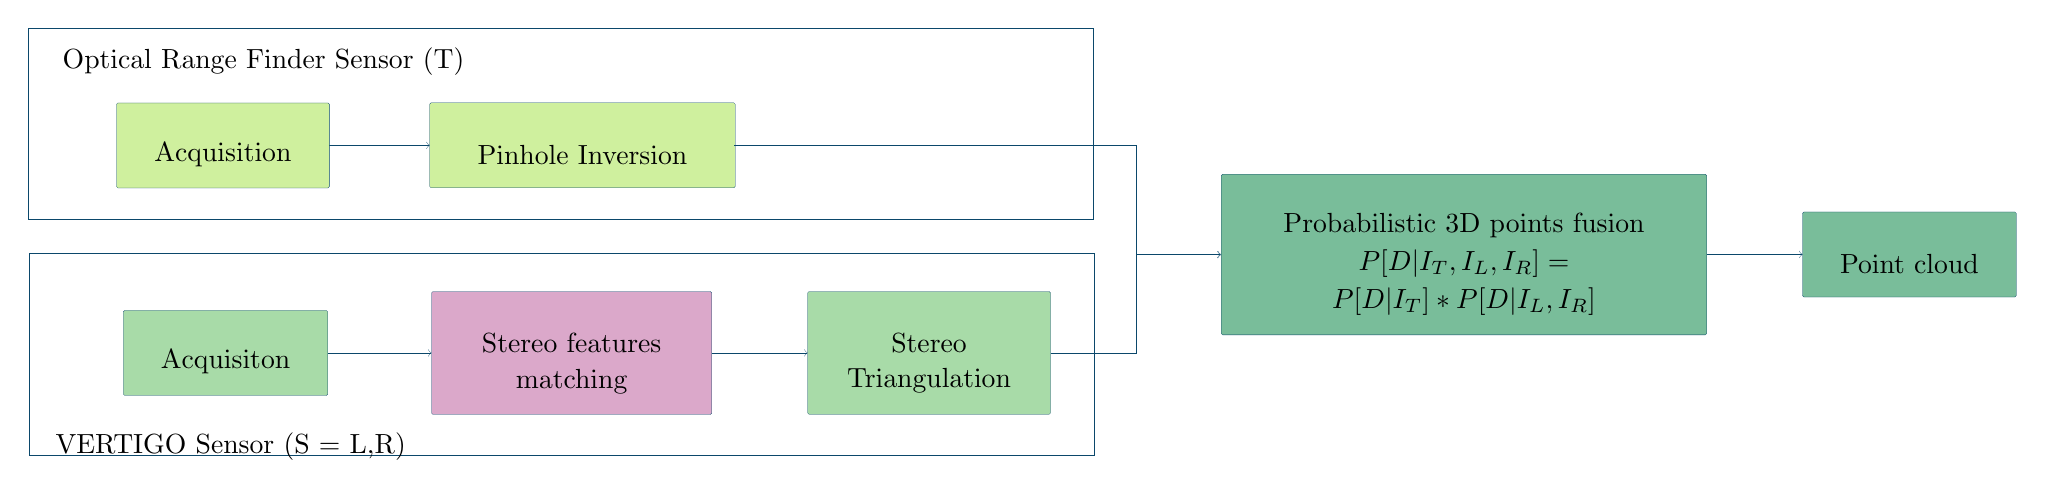
\begin{tikzpicture}
\pgftransformxscale{0.600000}
\pgftransformyscale{-0.600000}
\definecolor{dialinecolor}{rgb}{0.000000, 0.000000, 0.000000}
\pgfsetstrokecolor{dialinecolor}
\definecolor{dialinecolor}{rgb}{1.000000, 1.000000, 1.000000}
\pgfsetfillcolor{dialinecolor}
\pgfsetlinewidth{0.100000\du}
\pgfsetdash{}{0pt}
{\pgfsetcornersarced{\pgfpoint{0.500000\du}{0.500000\du}}\definecolor{dialinecolor}{rgb}{0.811765, 0.941176, 0.619608}
\pgfsetfillcolor{dialinecolor}
\fill (14.962113\du,11.000000\du)--(14.962113\du,12.800000\du)--(21.427113\du,12.800000\du)--(21.427113\du,11.000000\du)--cycle;
}{\pgfsetcornersarced{\pgfpoint{0.500000\du}{0.500000\du}}\definecolor{dialinecolor}{rgb}{0.043137, 0.282353, 0.419608}
\pgfsetstrokecolor{dialinecolor}
\draw (14.962113\du,11.000000\du)--(14.962113\du,12.800000\du)--(21.427113\du,12.800000\du)--(21.427113\du,11.000000\du)--cycle;
}% setfont left to latex
\definecolor{dialinecolor}{rgb}{0.043137, 0.282353, 0.419608}
\pgfsetstrokecolor{dialinecolor}
\node at (18.194613\du,12.095000\du){Pinhole Inversion};
\pgfsetlinewidth{0.100000\du}
\pgfsetdash{}{0pt}
{\pgfsetcornersarced{\pgfpoint{0.500000\du}{0.500000\du}}\definecolor{dialinecolor}{rgb}{0.858824, 0.658824, 0.792157}
\pgfsetfillcolor{dialinecolor}
\fill (15.000000\du,14.995264\du)--(15.000000\du,17.595264\du)--(20.932500\du,17.595264\du)--(20.932500\du,14.995264\du)--cycle;
}{\pgfsetcornersarced{\pgfpoint{0.500000\du}{0.500000\du}}\definecolor{dialinecolor}{rgb}{0.043137, 0.282353, 0.419608}
\pgfsetstrokecolor{dialinecolor}
\draw (15.000000\du,14.995264\du)--(15.000000\du,17.595264\du)--(20.932500\du,17.595264\du)--(20.932500\du,14.995264\du)--cycle;
}% setfont left to latex
\definecolor{dialinecolor}{rgb}{0.043137, 0.282353, 0.419608}
\pgfsetstrokecolor{dialinecolor}
\node at (17.966250\du,16.090264\du){Stereo features};
% setfont left to latex
\definecolor{dialinecolor}{rgb}{0.043137, 0.282353, 0.419608}
\pgfsetstrokecolor{dialinecolor}
\node at (17.966250\du,16.890264\du){ matching};
\pgfsetlinewidth{0.100000\du}
\pgfsetbuttcap
\pgfsetdash{}{0pt}
{
\definecolor{dialinecolor}{rgb}{0.043137, 0.282353, 0.419608}
\pgfsetfillcolor{dialinecolor}
% was here!!!
\pgfsetarrowsend{to}
\definecolor{dialinecolor}{rgb}{0.043137, 0.282353, 0.419608}
\pgfsetstrokecolor{dialinecolor}
\draw (12.837930\du,11.901712\du)--(13.900022\du,11.901712\du)--(13.900022\du,11.900000\du)--(14.962113\du,11.900000\du);
}
% setfont left to latex
\pgfsetlinewidth{0.100000\du}
\pgfsetbuttcap
\pgfsetdash{}{0pt}
{
\definecolor{dialinecolor}{rgb}{0.043137, 0.282353, 0.419608}
\pgfsetfillcolor{dialinecolor}
% was here!!!
\pgfsetarrowsend{to}
\definecolor{dialinecolor}{rgb}{0.043137, 0.282353, 0.419608}
\pgfsetstrokecolor{dialinecolor}
\draw (12.804756\du,16.294325\du)--(13.525000\du,16.294325\du)--(13.525000\du,16.295264\du)--(15.000000\du,16.295264\du);
}
% setfont left to latex
\pgfsetlinewidth{0.100000\du}
\pgfsetdash{}{0pt}
{\pgfsetcornersarced{\pgfpoint{0.500000\du}{0.500000\du}}\definecolor{dialinecolor}{rgb}{0.474510, 0.741176, 0.603922}
\pgfsetfillcolor{dialinecolor}
\fill (31.715151\du,12.511789\du)--(31.715151\du,15.911789\du)--(41.992651\du,15.911789\du)--(41.992651\du,12.511789\du)--cycle;
}{\pgfsetcornersarced{\pgfpoint{0.500000\du}{0.500000\du}}\definecolor{dialinecolor}{rgb}{0.043137, 0.282353, 0.419608}
\pgfsetstrokecolor{dialinecolor}
\draw (31.715151\du,12.511789\du)--(31.715151\du,15.911789\du)--(41.992651\du,15.911789\du)--(41.992651\du,12.511789\du)--cycle;
}% setfont left to latex
\definecolor{dialinecolor}{rgb}{0.043137, 0.282353, 0.419608}
\pgfsetstrokecolor{dialinecolor}
\node at (36.853901\du,13.606789\du){Probabilistic 3D points fusion};
% setfont left to latex
\definecolor{dialinecolor}{rgb}{0.043137, 0.282353, 0.419608}
\pgfsetstrokecolor{dialinecolor}
\node at (36.853901\du,14.406789\du){$P[D|I_T, I_L, I_R] =$};
% setfont left to latex
\definecolor{dialinecolor}{rgb}{0.043137, 0.282353, 0.419608}
\pgfsetstrokecolor{dialinecolor}
\node at (36.853901\du,15.206789\du){$P[D|I_T] * P[D|I_L,I_R]$};
\pgfsetlinewidth{0.100000\du}
\pgfsetdash{}{0pt}
{\pgfsetcornersarced{\pgfpoint{0.500000\du}{0.500000\du}}\definecolor{dialinecolor}{rgb}{0.658824, 0.858824, 0.658824}
\pgfsetfillcolor{dialinecolor}
\fill (22.961654\du,14.994000\du)--(22.961654\du,17.594000\du)--(28.101654\du,17.594000\du)--(28.101654\du,14.994000\du)--cycle;
}{\pgfsetcornersarced{\pgfpoint{0.500000\du}{0.500000\du}}\definecolor{dialinecolor}{rgb}{0.043137, 0.282353, 0.419608}
\pgfsetstrokecolor{dialinecolor}
\draw (22.961654\du,14.994000\du)--(22.961654\du,17.594000\du)--(28.101654\du,17.594000\du)--(28.101654\du,14.994000\du)--cycle;
}% setfont left to latex
\definecolor{dialinecolor}{rgb}{0.043137, 0.282353, 0.419608}
\pgfsetstrokecolor{dialinecolor}
\node at (25.531654\du,16.089000\du){Stereo};
% setfont left to latex
\definecolor{dialinecolor}{rgb}{0.043137, 0.282353, 0.419608}
\pgfsetstrokecolor{dialinecolor}
\node at (25.531654\du,16.889000\du){Triangulation};
\pgfsetlinewidth{0.100000\du}
\pgfsetdash{}{0pt}
{\pgfsetcornersarced{\pgfpoint{0.500000\du}{0.500000\du}}\definecolor{dialinecolor}{rgb}{0.811765, 0.941176, 0.619608}
\pgfsetfillcolor{dialinecolor}
\fill (8.332930\du,11.001712\du)--(8.332930\du,12.801712\du)--(12.837930\du,12.801712\du)--(12.837930\du,11.001712\du)--cycle;
}{\pgfsetcornersarced{\pgfpoint{0.500000\du}{0.500000\du}}\definecolor{dialinecolor}{rgb}{0.043137, 0.282353, 0.419608}
\pgfsetstrokecolor{dialinecolor}
\draw (8.332930\du,11.001712\du)--(8.332930\du,12.801712\du)--(12.837930\du,12.801712\du)--(12.837930\du,11.001712\du)--cycle;
}% setfont left to latex
\definecolor{dialinecolor}{rgb}{0.043137, 0.282353, 0.419608}
\pgfsetstrokecolor{dialinecolor}
\node at (10.585430\du,12.096712\du){Acquisition};
\pgfsetlinewidth{0.100000\du}
\pgfsetdash{}{0pt}
{\pgfsetcornersarced{\pgfpoint{0.500000\du}{0.500000\du}}\definecolor{dialinecolor}{rgb}{0.658824, 0.858824, 0.658824}
\pgfsetfillcolor{dialinecolor}
\fill (8.477256\du,15.394325\du)--(8.477256\du,17.194325\du)--(12.804756\du,17.194325\du)--(12.804756\du,15.394325\du)--cycle;
}{\pgfsetcornersarced{\pgfpoint{0.500000\du}{0.500000\du}}\definecolor{dialinecolor}{rgb}{0.043137, 0.282353, 0.419608}
\pgfsetstrokecolor{dialinecolor}
\draw (8.477256\du,15.394325\du)--(8.477256\du,17.194325\du)--(12.804756\du,17.194325\du)--(12.804756\du,15.394325\du)--cycle;
}% setfont left to latex
\definecolor{dialinecolor}{rgb}{0.043137, 0.282353, 0.419608}
\pgfsetstrokecolor{dialinecolor}
\node at (10.641006\du,16.489325\du){Acquisiton};
\pgfsetlinewidth{0.100000\du}
\pgfsetdash{}{0pt}
{\pgfsetcornersarced{\pgfpoint{0.500000\du}{0.500000\du}}\definecolor{dialinecolor}{rgb}{0.474510, 0.741176, 0.603922}
\pgfsetfillcolor{dialinecolor}
\fill (44.018906\du,13.310344\du)--(44.018906\du,15.110344\du)--(48.543906\du,15.110344\du)--(48.543906\du,13.310344\du)--cycle;
}{\pgfsetcornersarced{\pgfpoint{0.500000\du}{0.500000\du}}\definecolor{dialinecolor}{rgb}{0.043137, 0.282353, 0.419608}
\pgfsetstrokecolor{dialinecolor}
\draw (44.018906\du,13.310344\du)--(44.018906\du,15.110344\du)--(48.543906\du,15.110344\du)--(48.543906\du,13.310344\du)--cycle;
}% setfont left to latex
\definecolor{dialinecolor}{rgb}{0.043137, 0.282353, 0.419608}
\pgfsetstrokecolor{dialinecolor}
\node at (46.281406\du,14.405344\du){Point cloud};
\pgfsetlinewidth{0.100000\du}
\pgfsetbuttcap
\pgfsetdash{}{0pt}
{
\definecolor{dialinecolor}{rgb}{0.043137, 0.282353, 0.419608}
\pgfsetfillcolor{dialinecolor}
% was here!!!
\pgfsetarrowsend{to}
\definecolor{dialinecolor}{rgb}{0.043137, 0.282353, 0.419608}
\pgfsetstrokecolor{dialinecolor}
\draw (20.932500\du,16.295264\du)--(21.947077\du,16.295264\du)--(21.947077\du,16.294000\du)--(22.961654\du,16.294000\du);
}
% setfont left to latex
\pgfsetlinewidth{0.150000\du}
\pgfsetdash{}{0pt}
\pgfsetdash{}{0pt}
\pgfsetmiterjoin
\definecolor{dialinecolor}{rgb}{0.043137, 0.282353, 0.419608}
\pgfsetstrokecolor{dialinecolor}
\draw (6.456786\du,9.414155\du)--(6.456786\du,13.468052\du)--(28.999486\du,13.468052\du)--(28.999486\du,9.414155\du)--cycle;
\pgfsetlinewidth{0.150000\du}
\pgfsetdash{}{0pt}
\pgfsetdash{}{0pt}
\pgfsetmiterjoin
\definecolor{dialinecolor}{rgb}{0.043137, 0.282353, 0.419608}
\pgfsetstrokecolor{dialinecolor}
\draw (6.482533\du,14.183341\du)--(6.482533\du,18.469122\du)--(29.025233\du,18.469122\du)--(29.025233\du,14.183341\du)--cycle;
\pgfsetlinewidth{0.100000\du}
\pgfsetbuttcap
\pgfsetdash{}{0pt}
{
\definecolor{dialinecolor}{rgb}{0.043137, 0.282353, 0.419608}
\pgfsetfillcolor{dialinecolor}
% was here!!!
\pgfsetarrowsend{to}
\definecolor{dialinecolor}{rgb}{0.043137, 0.282353, 0.419608}
\pgfsetstrokecolor{dialinecolor}
\draw (21.412906\du,11.900000\du)--(29.904036\du,11.900000\du)--(29.904036\du,14.211789\du)--(31.700944\du,14.211789\du);
}
% setfont left to latex
\pgfsetlinewidth{0.100000\du}
\pgfsetbuttcap
\pgfsetdash{}{0pt}
{
\definecolor{dialinecolor}{rgb}{0.043137, 0.282353, 0.419608}
\pgfsetfillcolor{dialinecolor}
% was here!!!
\pgfsetarrowsend{to}
\definecolor{dialinecolor}{rgb}{0.043137, 0.282353, 0.419608}
\pgfsetstrokecolor{dialinecolor}
\draw (28.101654\du,16.294000\du)--(29.908403\du,16.294000\du)--(29.908403\du,14.211789\du)--(31.715151\du,14.211789\du);
}
% setfont left to latex
% setfont left to latex
\definecolor{dialinecolor}{rgb}{0.043137, 0.282353, 0.419608}
\pgfsetstrokecolor{dialinecolor}
\node[anchor=west] at (17.728136\du,11.441104\du){};
% setfont left to latex
\definecolor{dialinecolor}{rgb}{0.043137, 0.282353, 0.419608}
\pgfsetstrokecolor{dialinecolor}
\node[anchor=west] at (6.996674\du,10.124534\du){Optical Range Finder Sensor (T)};
% setfont left to latex
\definecolor{dialinecolor}{rgb}{0.043137, 0.282353, 0.419608}
\pgfsetstrokecolor{dialinecolor}
\node[anchor=west] at (6.845126\du,18.270216\du){VERTIGO Sensor (S = L,R)};
\pgfsetlinewidth{0.100000\du}
\pgfsetbuttcap
\pgfsetdash{}{0pt}
{
\definecolor{dialinecolor}{rgb}{0.043137, 0.282353, 0.419608}
\pgfsetfillcolor{dialinecolor}
% was here!!!
\pgfsetarrowsend{to}
\definecolor{dialinecolor}{rgb}{0.043137, 0.282353, 0.419608}
\pgfsetstrokecolor{dialinecolor}
\draw (41.992651\du,14.211789\du)--(43.005779\du,14.211789\du)--(43.005779\du,14.210344\du)--(44.018906\du,14.210344\du);
}
% setfont left to latex
\end{tikzpicture}

		}
	\end{center}
	\caption{The physical sensors of the \gls{INSPECT} project are represented with their software in a \textit{common representation format} which enables a probabilistic fusion \cite{multi_sensors_fusion}}\label{fig:sensors}
\end{figure}

If we adopt the representation and the notation in \cite{multi_sensors_fusion}, a \textit{sensor} $E$ is a system (hardware + software) characterized by its state, function, performances, output and energy type. In this case, we then consider two external sensors dedicated to navigation through 3D environment reconstruction whose output is a 3D point cloud combined with a monochromatic image (figure \ref{fig:sensors}). The performances are summarized in table \ref{table:perf}

\begin{center}
\begin{longtable}{|l|p{5.5cm}|p{5.5cm}|}
\hline
Performance & ORF & VERTIGO Sensors\\
\hline
Accuracy & Omnipresent noise & Good (if results)\\
\hline
Repeatability & Very good & Very good\\
\hline
Linearity & Non-linear with object speed and distance & Non-linear with object textures\\
\hline
Sensitivity & Sensible to luminous noise, saturation and movement & Sensible to the lack of texture in the environment\\
\hline
Resolution & Medium spatial resolution and good temporal resolution & Good spatial resolution and bad temporal resolution (computation)\\
\hline
Reliability & A result is guaranteed (but with variable quality) & Result not always guaranteed \\
\hline
Range & Very limited & Good\\
\hline
\caption{Performances of the two sensors according to the notation in \cite{multi_sensors_fusion}}\label{table:perf}
\end{longtable}
\end{center}

For each sensor, we can also define a \textit{sensor observation} $O$:
\begin{equation}
O = \langle E, \mathbf{x}, t, \mathbf{y}, \mathbf{\Delta y} \rangle
\end{equation}
Where:
\begin{itemize*}
\item $E$: the entity name which include the name of the physical property measured by the sensors as well as the units. Here, we measure \textit{3D point clouds} with their luminous intensity. In this work, we do not try to measure a spectral intensity as we will do next when the thermo-graphic camera will be added, we just need to know if the point exists or not (boolean measurement)
\item $\mathbf{x}$: the spatial location of the measurement (the 3D coordinates of each point in an absolute coordinate system)
\item $\mathbf{y}$: the value of the measurement (exists or not)
\item $\mathbf{\Delta y}$: a generic term which includes many types of errors including measurement, calibration, location,...
\end{itemize*}

\subsubsection{Fusion}
To perform fusion between them, the two \textit{sensors observations} must be represented in the same \textit{common representational format} which means we shall perform:
\begin{itemize*}
\item \textit{Spatial Alignment}: This process also called \textit{registration} consists of matching both sensors point clouds together. This task is one of the most important in the fusion and involves \textit{triangulation} and \textit{re-projection} using the calibration matrices as discussed in sections \ref{sec:stereo_camera} and \ref{sec:ORF_model}. In this work, we will do:
\begin{center}
2D points in $T$ reference system $\Rightarrow$ Triangulation $\Rightarrow$ 3D points in $T$ $\Rightarrow$ 3D points in $L$ $\Rightarrow$ Projection $\Rightarrow$ 2D points in $L$ and $R$
\end{center}
\item \textit{Temporal Alignment}: It is the transformation of the local times $t$ to a common time axis. In this work, we can estimate the image acquisition to be synchronous between the two devices (a system of time stamps has been implemented to guarantee this approximation) and we will not focus on this point.
\item \textit{Sensor Value Normalization}: As explained in \cite{multi_sensors_fusion}, normalizing two sensors with different physical properties is generally done by converting them into \textit{a posteriori probabilities}. In that case, estimated outputs are given by the application of the Bayes theorem. Here we can assimilate the computation of a 3D cloud to the research of a depth distribution $D$ which will be estimated by the system as a distribution $\hat{D}$ which maximizes the probability:
\begin{equation}
\hat{D} =  \mathtt{arg}\enspace \mathsf{max}\,\mathit{P}[D|I_T, I_L, I_R] =  \mathtt{arg}\enspace \mathsf{max}\,\dfrac{\mathit{P}[I_T, I_L, I_R|D] \mathit{P}[D]}{\mathit{P}[I_T, I_L, I_R]}
\end{equation}
Since $\mathit{P}[I_T, I_L, I_R]$ is not $D$-dependent, it can be replaced by any constant without changing the problem. Within those constants, let choose $\mathit{P}[I_T] \mathit{P}[I_L, I_R]$:
\begin{equation}
\hat{D} = \mathtt{arg}\enspace \mathsf{max}\,\dfrac{\mathit{P}[I_T, I_L, I_R|D] \mathit{P}[D]}{\mathit{P}[I_T] \mathit{P}[I_L, I_R]}
\end{equation}
As the camera depth distribution can be considered uniform, we can also write:
\begin{equation}
\hat{D} = \mathtt{arg}\enspace \mathsf{max}\,\dfrac{\mathit{P}[I_T, I_L, I_R|D] \mathit{P}[D]\mathit{P}[D]}{\mathit{P}[I_T] \mathit{P}[I_L, I_R]}
\end{equation}
One major hypothesis in the fusion is that $\{I_T, D\}$ and $\{I_L, I_R, D\}$ are independent \cite{stereo_tof_fusion_proba}. It leads to:
\begin{eqnarray}
\hat{D} & = & \mathtt{arg}\enspace \mathsf{max}\,\dfrac{\mathit{P}[I_T|D] \mathit{P}[D]}{\mathit{P}[I_T]}*\dfrac{\mathit{P}[I_L, I_R|D] \mathit{P}[D]}{\mathit{P}[I_L, I_R]}\\
\hat{D} & = & \mathtt{arg}\enspace \mathsf{max}\,\mathit{P}[D|I_T]*\mathit{P}[D|I_L, I_R]
\end{eqnarray}

\end{itemize*}
Finally, a fusion algorithm is characterized in terms of representation, certainty, accuracy, completeness. They will be discussed again when the results are introduced in chapter \ref{chapter:results} but we can already say:
\begin{itemize*}
\item \textbf{Representation}: This feature characterizing the abstraction level increasse from the algorithm inputs (2D matrices) to the algorithm outputs (3D point clouds).
\item \textbf{Certainty}: The gain in measurement certainty illustrates the growth between $\mathit{P}[D|I_T]$ and $\mathit{P}[D|I_L, I_R]$ on one hand and $\mathit{P}[D|I_T, I_L, I_R]$ on the other hand. It will be discussed in chapter \ref{chapter:results}.
\item \textbf{Accuracy}: The gain in measurement accuracy before and after the fusion will be discussed in chapter \ref{chapter:results}.
\item \textbf{Completeness}: The completeness will be affected by the limited \gls{FoV} of each cameras and the geometry between them. This feature is environment-dependent and will depend on the target size and distance and the application we want to perform.
\end{itemize*}

\subsection{Architecture}
All the concepts above leads to the architecture in figure \ref{fig:fusion_arch} that shows the big scheme of the fusion algorithm implemented in this thesis. However, there is a big difference compared to figure \ref{fig:sensors}. Indeed, we want to avoid \textit{feature matching} between stereo images which leads to bad results in poor textured environment. To avoid this problem, the fusion architecture in \cite{stereo_tof_fusion_proba} is exploited. This will be discussed in chapter \ref{chapter:results}.


\subsubsection{Determination of the Points Framed by all Cameras}
In order to perform \textit{registration}, the determination of the domain framed by both devices must be accomplished as the first step of the algorithm. We then only keep the points framed by the two cameras before proceeding to the fusion. Figure \ref{fig:geometry} shows the three devices \gls{FoV} in the $XZ$ plane. The hatched zone corresponds to the domain where fusion will take place. As we consider the three cameras have the same $Y$ coordinate, the $Y$ domain is given by the minimal \gls{FoV}. Basic analytical calculations give:
\begin{eqnarray}
z_i & \in & \Big[min\Big(\frac{t_{TR}\,\mathsf{tan}(\rho)\,\mathsf{tan}(\tau)}{\mathsf{tan}(\rho) + \mathsf{tan}(\tau)}, range_{min}\Big);\,range_{max}\Big]\\
x_i & \in & \Big[\dfrac{-z_i-t_{TR}\mathsf{tan}(\rho)}{\mathsf{tan}(\rho)};\,\dfrac{z_i}{\mathsf{tan}(\rho)}\Big]\\
y_i & \in & \Big[min\Big(\dfrac{-z_i}{\mathsf{tan}(\rho)}, \dfrac{-z_i}{\mathsf{tan}(\tau)}\Big);\,min\Big(\dfrac{z_i}{\mathsf{tan}(\rho)}, \dfrac{z_i}{\mathsf{tan}(\tau)}\Big)\Big]
\end{eqnarray}

% Figure geometry
\begin{figure}[!htt]
	\begin{center}
		\includegraphics[width=10cm]{img/geometry.png}
		\caption{The region framed by the three cameras depends on the \textit{baseline} between the cameras as well as their \gls{FoV}}
		\label{fig:geometry}
	\end{center}
\end{figure}


\subsubsection{Optical Range Finder Noise Model}
According to \cite{orf_calib} and \cite{stereo_tof_fusion_proba}, the error in the depth measurement $\hat{D}_T$ for each pixel captured by the \gls{ORF} camera can be mainly described as the sum of the following components:
\begin{itemize*}
\item A \textit{thermal noise} with a Gaussian distribution
\item A \textit{quantization error}
\item A \textit{photon shot noise} with a Poisson distribution
\item A \textit{scattering generated noise} especially in presence of discontinuities
\end{itemize*}
According to the same sources, they consider the \textit{quantization error} and the \textit{photon shot noise} can be neglected in front of the \textit{thermal noise}. The latter can be represented by a Normal distribution around the measured depth:
\begin{equation}
\mathcal{N}(d_T^i, \sigma_t^2)
\end{equation}
Where $\sigma_t$ is inversely proportional to the confidence of the pixel given in the pixel map $C_T$. In our experiment set, we selected a factor $\sigma_t^2 = (range_{max} - C_T)/10$.
Concerning the scattering noise, \cite{orf_scattering} shows that it could also be expressed with a normal distribution:
\begin{equation}
\mathcal{N}(d_T^i, \sigma_s^2)
\end{equation}
Where $\sigma_s^2$ is the variance of the measured depths in the second order neighborhood of the considered pixel $p_T$.
Finally, the thermal noise is neglected near discontinuities and scattering noise far from discontinuities which gives:
\begin{equation}
\mathit{P}[d^i|I_T] \sim \mathcal{N}(d_T^i, \sigma_w^2)
\end{equation}
Where:
\begin{equation}
\sigma_w = \mathsf{max}(\sigma_t, \sigma_s)
\end{equation}

\subsubsection{Probabilistic Space Discretization}
Once the noise has been determined for each pixel, we can assume the real depth is situated at maximum $3 \sigma_w$ from the measured depth:
\begin{equation}
d^i \in [d_T^i - 3 \sigma_w;\,d_T^i + 3 \sigma_w]
\end{equation}

% figure orf_normal
\begin{figure}[H]
	\begin{center}
		\includegraphics[width=12cm]{img/orf_normal.png}
		\caption{The interval around the measured depth $d_T^i$ is divided in $j$ steps of length $\epsilon_D$}
		\label{fig:orf_normal}
	\end{center}
\end{figure}


As presented in figure \ref{fig:orf_normal}, this interval is then discretized around $\hat{D}_T$ with a step equal to the stereoscopic accuracy sub-sampled by a factor $k_int$ ($k_{int} = 4$ in this work). In \cite{stereo_resolution} and \cite{stereo_resolution_2}, this resolution is equal to:
\begin{equation}
\label{eq:stereo_acc}
\epsilon_D = \dfrac{D^2}{b\, f}\,\epsilon_p
\end{equation}
Where $D$ is the depth, $b$ is the \textit{baseline} between $L$ and $R$ cameras, $f$ is the focal length (assumed to be the same for $L$ and $R$) and $\epsilon_p$ is the distance between two pixels on the camera ($6 \mu m$ for \gls{VERTIGO}) as shown in figure \ref{fig:cam_stereo_resolution}.

% figure cam_stereo_resolution
\begin{figure}[H]
	\begin{center}
		\includegraphics[width=6cm]{img/cam_stereo_resolution.png}
		\caption{The theoretical depth error for stereo devices depends on the depth $D$, the baseline between cameras $b$, the pixel size $\epsilon_p$ and the focal length $f$}
		\label{fig:cam_stereo_resolution}
	\end{center}
\end{figure}

\subsubsection{Optical Range Finder Probabilistic Model}
For each pixel of the depth map $d^i$ ($i=1..n$), we have constructed a sample of $j$ points $d^{i,j}$ ($j=1..m$) which are the candidates to represent the true depth $D$. As explained in section \ref{subsec:fusion:overview}, the next step to perform fusion consists of determining $\mathit{P}[d^i = d^{i,j} |I_T]$ and $\mathit{P}[d^i = d^{i,j}|I_L, I_R]$.
As shown previously, we can directly write:
\begin{equation}
\mathit{P}[d^i = d^{i,j}|I_T] = \frac{1}{\sigma_w^i \sqrt{2\pi} } e^{ -\frac{(d^{i,j} - d^i)^2}{2{\sigma_w^i}^2}}
\end{equation}

\subsubsection{Stereoscopic Cameras Probabilistic Model}
The computation of the probability $\mathit{P}[d^i = d^{i,j}|I_L, I_R]$ involves the re-projection of the 3D coordinates obtained for all $d^{i,j}$ from the \gls{ORF} (figure \ref{fig:stereo_proba}). It is a way to avoid straightforward feature matching whose results depend on the texture level of the scene as explained previously.

% Figure stereo_proba
\begin{figure}[H]
	\begin{center}
		\includegraphics[width=12cm]{img/cam_stereo_proba.png}
		\caption{For each pixel, each $P_T^{i,j}$ is reprojected in $L$ and $R$ image planes. From those coordinates, a probability will be established to correct the depth measured by the \gls{ORF}}
		\label{fig:stereo_proba}
	\end{center}
\end{figure}

After this re-projection, the probability is computed as an exponential distribution which decreases according to a factor $c_{i,j}$ representing the degree of likeness between a point $P^{i,j}$ projected in $L$ and $R$:
\begin{equation}
\mathit{P}[d^i = d^{i,j}|I_L, I_R] = e^{\dfrac{-c_{i,j}}{\sigma_w^i}}
\end{equation}
In this way, when we project all the $j$ points discretized from the \gls{ORF} Normal probability of a pixel $i$, we can compute a degree likeness for each pair in $L$ and $R$. As a pixel is very tiny, a small offset could incur a big mismatch between $L$ and $R$ projection, that is why we consider a rectangular window of size $(k,l)$ around this point and we compute $c_{i,j}$ as a truncated sum of the absolute difference (\textit{L1-norm}) between each point of the window \cite{stereo_windowing}:
\begin{equation}
c_{i,j} = \mathsf{min}\Big\{\sum_k \sum_l\, \big|I_L(u_{i,j} + k, v_{i,j} + l) - I_R(u_{i,j} + k, v_{i,j} + l)\big|\,,\,thresh\Big\}
\end{equation}
Where the value $thresh$ will be discussed in the results.

\subsubsection{Joint Probability Computation}
For each pixel $i$, we deduce the joint probability:
\begin{equation}
\mathit{P}[d^i = d^{i,j}|I_T,I_L, I_R] = \mathit{P}[d^i = d^{i,j} |I_T]\,\,*\,\,\mathit{P}[d^i = d^{i,j}|I_L, I_R]
\end{equation}

\subsubsection{Depth Estimation Selection}
To create an improved 3D map, the last step consists of selecting the maximal probability in the selected interval for each pixel $i$:
\begin{equation}
\hat{d}_i = \mathsf{max}_{\,j} \Big\{\mathit{P}[d^i = d^{i,j}|I_T,I_L, I_R]\Big\}
\end{equation}

\subsubsection{3D Coordinates Computation}
From the variables $(u_T^i, v_T^i, \hat{d}_i)$, we recover $\hat{P}^i = (\hat{x}^i, \hat{y}^i, \hat{z}^i)$ by inverting the pinhole equation as described in \ref{subsubsec:orf_pinhole_inverstion}.

\subsubsection{Point Cloud Creation}
As a last step, a point cloud $\hat{\mathbf{P}}$ is composed by the assembly of every pixel $\hat{P}^i$

% Figure arch
\begin{figure}[!htt] 
	\begin{center}
		{\scalefont{0.5}
		% Graphic for TeX using PGF
% Title: /home/gabs48/mit/thesis/graphic/arch.dia
% Creator: Dia v0.97.2
% CreationDate: Fri Oct 10 17:15:52 2014
% For: gabs48
% \usepackage{tikz}
% The following commands are not supported in PSTricks at present
% We define them conditionally, so when they are implemented,
% this pgf file will use them.
\ifx\du\undefined
  \newlength{\du}
\fi
\setlength{\du}{15\unitlength}
\begin{tikzpicture}
\pgftransformxscale{0.600000}
\pgftransformyscale{-0.600000}
\definecolor{dialinecolor}{rgb}{0.000000, 0.000000, 0.000000}
\pgfsetstrokecolor{dialinecolor}
\definecolor{dialinecolor}{rgb}{1.000000, 1.000000, 1.000000}
\pgfsetfillcolor{dialinecolor}
\pgfsetlinewidth{0.100000\du}
\pgfsetdash{}{0pt}
{\pgfsetcornersarced{\pgfpoint{0.500000\du}{0.500000\du}}\definecolor{dialinecolor}{rgb}{0.474510, 0.741176, 0.603922}
\pgfsetfillcolor{dialinecolor}
\fill (8.393256\du,11.632739\du)--(8.393256\du,15.032739\du)--(24.693256\du,15.032739\du)--(24.693256\du,11.632739\du)--cycle;
}{\pgfsetcornersarced{\pgfpoint{0.500000\du}{0.500000\du}}\definecolor{dialinecolor}{rgb}{0.043137, 0.282353, 0.419608}
\pgfsetstrokecolor{dialinecolor}
\draw (8.393256\du,11.632739\du)--(8.393256\du,15.032739\du)--(24.693256\du,15.032739\du)--(24.693256\du,11.632739\du)--cycle;
}% setfont left to latex
\definecolor{dialinecolor}{rgb}{0.043137, 0.282353, 0.419608}
\pgfsetstrokecolor{dialinecolor}
\node at (16.543256\du,12.727739\du){- Calculate $\sigma_t^i = f(C_T^i)$};
% setfont left to latex
\definecolor{dialinecolor}{rgb}{0.043137, 0.282353, 0.419608}
\pgfsetstrokecolor{dialinecolor}
\node at (16.543256\du,13.527739\du){- Calculate $\sigma_s^i$ as the second order variance around $p_T^{i}$};
% setfont left to latex
\definecolor{dialinecolor}{rgb}{0.043137, 0.282353, 0.419608}
\pgfsetstrokecolor{dialinecolor}
\node at (16.543256\du,14.327739\du){- Calculate $\sigma_s^i = \mathsf{max}(\sigma_t^i, \sigma_s^i)$};
\definecolor{dialinecolor}{rgb}{0.658824, 0.858824, 0.658824}
\pgfsetfillcolor{dialinecolor}
\pgfpathellipse{\pgfpoint{42.058077\du}{1.812780\du}}{\pgfpoint{9.090108\du}{0\du}}{\pgfpoint{0\du}{1.527626\du}}
\pgfusepath{fill}
\pgfsetlinewidth{0.150000\du}
\pgfsetdash{}{0pt}
\pgfsetdash{}{0pt}
\definecolor{dialinecolor}{rgb}{0.043137, 0.282353, 0.419608}
\pgfsetstrokecolor{dialinecolor}
\pgfpathellipse{\pgfpoint{42.058077\du}{1.812780\du}}{\pgfpoint{9.090108\du}{0\du}}{\pgfpoint{0\du}{1.527626\du}}
\pgfusepath{stroke}
\definecolor{dialinecolor}{rgb}{0.811765, 0.941176, 0.619608}
\pgfsetfillcolor{dialinecolor}
\fill (29.385659\du,3.147960\du)--(38.634070\du,5.623995\du)--(29.385659\du,8.100030\du)--(20.137247\du,5.623995\du)--cycle;
\pgfsetlinewidth{0.150000\du}
\pgfsetdash{}{0pt}
\pgfsetdash{}{0pt}
\pgfsetmiterjoin
\definecolor{dialinecolor}{rgb}{0.043137, 0.282353, 0.419608}
\pgfsetstrokecolor{dialinecolor}
\draw (29.385659\du,3.147960\du)--(38.634070\du,5.623995\du)--(29.385659\du,8.100030\du)--(20.137247\du,5.623995\du)--cycle;
% setfont left to latex
\definecolor{dialinecolor}{rgb}{0.043137, 0.282353, 0.419608}
\pgfsetstrokecolor{dialinecolor}
\node at (29.385659\du,5.018995\du){For each $p_T^i \in D_T$, $p_T^i ?\in \mathcal{D}$};
% setfont left to latex
\definecolor{dialinecolor}{rgb}{0.043137, 0.282353, 0.419608}
\pgfsetstrokecolor{dialinecolor}
\node at (29.385659\du,5.818995\du){where $\mathcal{D} = \{p_T^i\}$ : $p_T^i$ is also framed};
% setfont left to latex
\definecolor{dialinecolor}{rgb}{0.043137, 0.282353, 0.419608}
\pgfsetstrokecolor{dialinecolor}
\node at (29.385659\du,6.618995\du){by $I_L$ and $I_R$};
\definecolor{dialinecolor}{rgb}{0.658824, 0.858824, 0.658824}
\pgfsetfillcolor{dialinecolor}
\pgfpathellipse{\pgfpoint{29.387845\du}{-0.057395\du}}{\pgfpoint{2.216383\du}{0\du}}{\pgfpoint{0\du}{0.890342\du}}
\pgfusepath{fill}
\pgfsetlinewidth{0.150000\du}
\pgfsetdash{}{0pt}
\pgfsetdash{}{0pt}
\definecolor{dialinecolor}{rgb}{0.043137, 0.282353, 0.419608}
\pgfsetstrokecolor{dialinecolor}
\pgfpathellipse{\pgfpoint{29.387845\du}{-0.057395\du}}{\pgfpoint{2.216383\du}{0\du}}{\pgfpoint{0\du}{0.890342\du}}
\pgfusepath{stroke}
\pgfsetlinewidth{0.150000\du}
\pgfsetdash{}{0pt}
\pgfsetdash{}{0pt}
\pgfsetbuttcap
\pgfsetmiterjoin
\pgfsetlinewidth{0.150000\du}
\pgfsetbuttcap
\pgfsetmiterjoin
\pgfsetdash{}{0pt}
\definecolor{dialinecolor}{rgb}{0.811765, 0.941176, 0.619608}
\pgfsetfillcolor{dialinecolor}
\pgfpathmoveto{\pgfpoint{8.503452\du}{8.203952\du}}
\pgfpathlineto{\pgfpoint{19.225442\du}{8.203952\du}}
\pgfpathlineto{\pgfpoint{17.081044\du}{6.253952\du}}
\pgfpathlineto{\pgfpoint{10.647850\du}{6.253952\du}}
\pgfpathlineto{\pgfpoint{8.503452\du}{8.203952\du}}
\pgfusepath{fill}
\definecolor{dialinecolor}{rgb}{0.043137, 0.282353, 0.419608}
\pgfsetstrokecolor{dialinecolor}
\pgfpathmoveto{\pgfpoint{8.503452\du}{8.203952\du}}
\pgfpathlineto{\pgfpoint{19.225442\du}{8.203952\du}}
\pgfpathlineto{\pgfpoint{17.081044\du}{6.253952\du}}
\pgfpathlineto{\pgfpoint{10.647850\du}{6.253952\du}}
\pgfpathlineto{\pgfpoint{8.503452\du}{8.203952\du}}
\pgfusepath{stroke}
% setfont left to latex
\definecolor{dialinecolor}{rgb}{0.043137, 0.282353, 0.419608}
\pgfsetstrokecolor{dialinecolor}
\node at (13.864447\du,7.028952\du){For each $p_i \in \mathcal{D}$};
% setfont left to latex
\definecolor{dialinecolor}{rgb}{0.043137, 0.282353, 0.419608}
\pgfsetstrokecolor{dialinecolor}
\node at (13.864447\du,7.828952\du){where $p^i = (u_T^i, v_T^i, d_T^i)$};
\pgfsetlinewidth{0.100000\du}
\pgfsetdash{}{0pt}
{\pgfsetcornersarced{\pgfpoint{0.500000\du}{0.500000\du}}\definecolor{dialinecolor}{rgb}{0.474510, 0.741176, 0.603922}
\pgfsetfillcolor{dialinecolor}
\fill (8.527961\du,17.402406\du)--(8.527961\du,20.802406\du)--(24.550461\du,20.802406\du)--(24.550461\du,17.402406\du)--cycle;
}{\pgfsetcornersarced{\pgfpoint{0.500000\du}{0.500000\du}}\definecolor{dialinecolor}{rgb}{0.043137, 0.282353, 0.419608}
\pgfsetstrokecolor{dialinecolor}
\draw (8.527961\du,17.402406\du)--(8.527961\du,20.802406\du)--(24.550461\du,20.802406\du)--(24.550461\du,17.402406\du)--cycle;
}% setfont left to latex
\definecolor{dialinecolor}{rgb}{0.043137, 0.282353, 0.419608}
\pgfsetstrokecolor{dialinecolor}
\node at (16.539211\du,18.497406\du){Create the interval $[d_T^i - 3 \sigma_w;\,d_T^i + 3 \sigma_w]$};
% setfont left to latex
\definecolor{dialinecolor}{rgb}{0.043137, 0.282353, 0.419608}
\pgfsetstrokecolor{dialinecolor}
\node at (16.539211\du,19.297406\du){divided in m steps};
% setfont left to latex
\definecolor{dialinecolor}{rgb}{0.043137, 0.282353, 0.419608}
\pgfsetstrokecolor{dialinecolor}
\node at (16.539211\du,20.097406\du){of size $\epsilon_D/k_{int}$};
\pgfsetlinewidth{0.150000\du}
\pgfsetdash{}{0pt}
\pgfsetdash{}{0pt}
\pgfsetbuttcap
\pgfsetmiterjoin
\pgfsetlinewidth{0.150000\du}
\pgfsetbuttcap
\pgfsetmiterjoin
\pgfsetdash{}{0pt}
\definecolor{dialinecolor}{rgb}{0.811765, 0.941176, 0.619608}
\pgfsetfillcolor{dialinecolor}
\pgfpathmoveto{\pgfpoint{4.471471\du}{25.824234\du}}
\pgfpathlineto{\pgfpoint{28.590841\du}{25.824234\du}}
\pgfpathlineto{\pgfpoint{23.766967\du}{23.874234\du}}
\pgfpathlineto{\pgfpoint{9.295345\du}{23.874234\du}}
\pgfpathlineto{\pgfpoint{4.471471\du}{25.824234\du}}
\pgfusepath{fill}
\definecolor{dialinecolor}{rgb}{0.043137, 0.282353, 0.419608}
\pgfsetstrokecolor{dialinecolor}
\pgfpathmoveto{\pgfpoint{4.471471\du}{25.824234\du}}
\pgfpathlineto{\pgfpoint{28.590841\du}{25.824234\du}}
\pgfpathlineto{\pgfpoint{23.766967\du}{23.874234\du}}
\pgfpathlineto{\pgfpoint{9.295345\du}{23.874234\du}}
\pgfpathlineto{\pgfpoint{4.471471\du}{25.824234\du}}
\pgfusepath{stroke}
% setfont left to latex
\definecolor{dialinecolor}{rgb}{0.043137, 0.282353, 0.419608}
\pgfsetstrokecolor{dialinecolor}
\node at (16.531156\du,24.649234\du){For each $p_T^{i,j} \in d_T^i - 3 \sigma_w;\,d_T^i + 3 \sigma_w]$};
% setfont left to latex
\definecolor{dialinecolor}{rgb}{0.043137, 0.282353, 0.419608}
\pgfsetstrokecolor{dialinecolor}
\node at (16.531156\du,25.449234\du){where $p_T^{i,j} = (u_T^i, v_T^i, d_T^{i,j})$ and $j=1..m$};
\pgfsetlinewidth{0.100000\du}
\pgfsetdash{}{0pt}
{\pgfsetcornersarced{\pgfpoint{0.500000\du}{0.500000\du}}\definecolor{dialinecolor}{rgb}{0.474510, 0.741176, 0.603922}
\pgfsetfillcolor{dialinecolor}
\fill (4.228975\du,32.349730\du)--(4.228975\du,36.549730\du)--(22.608975\du,36.549730\du)--(22.608975\du,32.349730\du)--cycle;
}{\pgfsetcornersarced{\pgfpoint{0.500000\du}{0.500000\du}}\definecolor{dialinecolor}{rgb}{0.043137, 0.282353, 0.419608}
\pgfsetstrokecolor{dialinecolor}
\draw (4.228975\du,32.349730\du)--(4.228975\du,36.549730\du)--(22.608975\du,36.549730\du)--(22.608975\du,32.349730\du)--cycle;
}% setfont left to latex
\definecolor{dialinecolor}{rgb}{0.043137, 0.282353, 0.419608}
\pgfsetstrokecolor{dialinecolor}
\node at (13.418975\du,33.444730\du){Calculate};
% setfont left to latex
\definecolor{dialinecolor}{rgb}{0.043137, 0.282353, 0.419608}
\pgfsetstrokecolor{dialinecolor}
\node at (13.418975\du,34.244730\du){};
% setfont left to latex
\definecolor{dialinecolor}{rgb}{0.043137, 0.282353, 0.419608}
\pgfsetstrokecolor{dialinecolor}
\node at (13.418975\du,35.044730\du){$\mathit{P}[d^i = d^{i,j}|I_T] = \frac{1}{\sigma_w^i \sqrt{2\pi} } e^{ -\frac{(d^{i,j} - d^i)^2}{2{\sigma_w^i}^2}}$};
% setfont left to latex
\definecolor{dialinecolor}{rgb}{0.043137, 0.282353, 0.419608}
\pgfsetstrokecolor{dialinecolor}
\node at (13.418975\du,35.844730\du){};
\pgfsetlinewidth{0.100000\du}
\pgfsetdash{}{0pt}
{\pgfsetcornersarced{\pgfpoint{0.500000\du}{0.500000\du}}\definecolor{dialinecolor}{rgb}{0.474510, 0.741176, 0.603922}
\pgfsetfillcolor{dialinecolor}
\fill (28.220357\du,27.844371\du)--(28.220357\du,30.444371\du)--(34.950357\du,30.444371\du)--(34.950357\du,27.844371\du)--cycle;
}{\pgfsetcornersarced{\pgfpoint{0.500000\du}{0.500000\du}}\definecolor{dialinecolor}{rgb}{0.043137, 0.282353, 0.419608}
\pgfsetstrokecolor{dialinecolor}
\draw (28.220357\du,27.844371\du)--(28.220357\du,30.444371\du)--(34.950357\du,30.444371\du)--(34.950357\du,27.844371\du)--cycle;
}% setfont left to latex
\definecolor{dialinecolor}{rgb}{0.043137, 0.282353, 0.419608}
\pgfsetstrokecolor{dialinecolor}
\node at (31.585357\du,28.939371\du){Recover $u_L^{i,j}$, $v_L^{i,j}$,};
% setfont left to latex
\definecolor{dialinecolor}{rgb}{0.043137, 0.282353, 0.419608}
\pgfsetstrokecolor{dialinecolor}
\node at (31.585357\du,29.739371\du){$u_R^{i,j}$, $v_R^{i,j}$ in $I_L, I_R$};
\pgfsetlinewidth{0.100000\du}
\pgfsetdash{}{0pt}
{\pgfsetcornersarced{\pgfpoint{0.500000\du}{0.500000\du}}\definecolor{dialinecolor}{rgb}{0.474510, 0.741176, 0.603922}
\pgfsetfillcolor{dialinecolor}
\fill (24.126652\du,32.471767\du)--(24.126652\du,36.671767\du)--(38.989152\du,36.671767\du)--(38.989152\du,32.471767\du)--cycle;
}{\pgfsetcornersarced{\pgfpoint{0.500000\du}{0.500000\du}}\definecolor{dialinecolor}{rgb}{0.043137, 0.282353, 0.419608}
\pgfsetstrokecolor{dialinecolor}
\draw (24.126652\du,32.471767\du)--(24.126652\du,36.671767\du)--(38.989152\du,36.671767\du)--(38.989152\du,32.471767\du)--cycle;
}% setfont left to latex
\definecolor{dialinecolor}{rgb}{0.043137, 0.282353, 0.419608}
\pgfsetstrokecolor{dialinecolor}
\node at (31.557902\du,33.566767\du){Calculate};
% setfont left to latex
\definecolor{dialinecolor}{rgb}{0.043137, 0.282353, 0.419608}
\pgfsetstrokecolor{dialinecolor}
\node at (31.557902\du,34.366767\du){};
% setfont left to latex
\definecolor{dialinecolor}{rgb}{0.043137, 0.282353, 0.419608}
\pgfsetstrokecolor{dialinecolor}
\node at (31.557902\du,35.166767\du){$\mathit{P}[d^i = d^{i,j}|I_L, I_R] = e^{\dfrac{-c_{i,j}}{\sigma_w^i}}$};
% setfont left to latex
\definecolor{dialinecolor}{rgb}{0.043137, 0.282353, 0.419608}
\pgfsetstrokecolor{dialinecolor}
\node at (31.557902\du,35.966767\du){};
\pgfsetlinewidth{0.100000\du}
\pgfsetdash{}{0pt}
{\pgfsetcornersarced{\pgfpoint{0.500000\du}{0.500000\du}}\definecolor{dialinecolor}{rgb}{0.474510, 0.741176, 0.603922}
\pgfsetfillcolor{dialinecolor}
\fill (11.114189\du,38.215757\du)--(11.114189\du,40.815757\du)--(30.404189\du,40.815757\du)--(30.404189\du,38.215757\du)--cycle;
}{\pgfsetcornersarced{\pgfpoint{0.500000\du}{0.500000\du}}\definecolor{dialinecolor}{rgb}{0.043137, 0.282353, 0.419608}
\pgfsetstrokecolor{dialinecolor}
\draw (11.114189\du,38.215757\du)--(11.114189\du,40.815757\du)--(30.404189\du,40.815757\du)--(30.404189\du,38.215757\du)--cycle;
}% setfont left to latex
\definecolor{dialinecolor}{rgb}{0.043137, 0.282353, 0.419608}
\pgfsetstrokecolor{dialinecolor}
\node at (20.759189\du,39.310757\du){Calculate joint Probability :};
% setfont left to latex
\definecolor{dialinecolor}{rgb}{0.043137, 0.282353, 0.419608}
\pgfsetstrokecolor{dialinecolor}
\node at (20.759189\du,40.110757\du){                                              $P[d^{i,j}|I_T, I_L, I_R] = P[d^{i,j}|I_T] * P[d^{i,j}|I_L,I_R]$};
\pgfsetlinewidth{0.150000\du}
\pgfsetdash{}{0pt}
\pgfsetdash{}{0pt}
\pgfsetbuttcap
\pgfsetmiterjoin
\pgfsetlinewidth{0.150000\du}
\pgfsetbuttcap
\pgfsetmiterjoin
\pgfsetdash{}{0pt}
\definecolor{dialinecolor}{rgb}{0.811765, 0.941176, 0.619608}
\pgfsetfillcolor{dialinecolor}
\pgfpathmoveto{\pgfpoint{11.051951\du}{42.746384\du}}
\pgfpathlineto{\pgfpoint{30.463785\du}{42.746384\du}}
\pgfpathlineto{\pgfpoint{26.581418\du}{44.696384\du}}
\pgfpathlineto{\pgfpoint{14.934318\du}{44.696384\du}}
\pgfpathlineto{\pgfpoint{11.051951\du}{42.746384\du}}
\pgfusepath{fill}
\definecolor{dialinecolor}{rgb}{0.043137, 0.282353, 0.419608}
\pgfsetstrokecolor{dialinecolor}
\pgfpathmoveto{\pgfpoint{11.051951\du}{42.746384\du}}
\pgfpathlineto{\pgfpoint{30.463785\du}{42.746384\du}}
\pgfpathlineto{\pgfpoint{26.581418\du}{44.696384\du}}
\pgfpathlineto{\pgfpoint{14.934318\du}{44.696384\du}}
\pgfpathlineto{\pgfpoint{11.051951\du}{42.746384\du}}
\pgfusepath{stroke}
% setfont left to latex
\definecolor{dialinecolor}{rgb}{0.043137, 0.282353, 0.419608}
\pgfsetstrokecolor{dialinecolor}
\node at (20.757868\du,43.921384\du){Select $\hat{d}^i = \mathtt{arg}\enspace \mathsf{max}\,\mathit{P}[d^{i,j}|I_T, I_L, I_R]$};
\definecolor{dialinecolor}{rgb}{0.658824, 0.858824, 0.658824}
\pgfsetfillcolor{dialinecolor}
\pgfpathellipse{\pgfpoint{34.149677\du}{25.334284\du}}{\pgfpoint{2.216383\du}{0\du}}{\pgfpoint{0\du}{0.890342\du}}
\pgfusepath{fill}
\pgfsetlinewidth{0.150000\du}
\pgfsetdash{}{0pt}
\pgfsetdash{}{0pt}
\definecolor{dialinecolor}{rgb}{0.043137, 0.282353, 0.419608}
\pgfsetstrokecolor{dialinecolor}
\pgfpathellipse{\pgfpoint{34.149677\du}{25.334284\du}}{\pgfpoint{2.216383\du}{0\du}}{\pgfpoint{0\du}{0.890342\du}}
\pgfusepath{stroke}
\definecolor{dialinecolor}{rgb}{0.658824, 0.858824, 0.658824}
\pgfsetfillcolor{dialinecolor}
\pgfpathellipse{\pgfpoint{39.116990\du}{28.717865\du}}{\pgfpoint{2.216383\du}{0\du}}{\pgfpoint{0\du}{0.890342\du}}
\pgfusepath{fill}
\pgfsetlinewidth{0.150000\du}
\pgfsetdash{}{0pt}
\pgfsetdash{}{0pt}
\definecolor{dialinecolor}{rgb}{0.043137, 0.282353, 0.419608}
\pgfsetstrokecolor{dialinecolor}
\pgfpathellipse{\pgfpoint{39.116990\du}{28.717865\du}}{\pgfpoint{2.216383\du}{0\du}}{\pgfpoint{0\du}{0.890342\du}}
\pgfusepath{stroke}
\pgfsetlinewidth{0.150000\du}
\pgfsetdash{}{0pt}
\pgfsetdash{}{0pt}
\pgfsetbuttcap
\pgfsetmiterjoin
\pgfsetlinewidth{0.150000\du}
\pgfsetbuttcap
\pgfsetmiterjoin
\pgfsetdash{}{0pt}
\definecolor{dialinecolor}{rgb}{0.811765, 0.941176, 0.619608}
\pgfsetfillcolor{dialinecolor}
\pgfpathmoveto{\pgfpoint{27.521062\du}{47.902946\du}}
\pgfpathlineto{\pgfpoint{44.771062\du}{47.902946\du}}
\pgfpathlineto{\pgfpoint{41.321062\du}{49.852946\du}}
\pgfpathlineto{\pgfpoint{30.971062\du}{49.852946\du}}
\pgfpathlineto{\pgfpoint{27.521062\du}{47.902946\du}}
\pgfusepath{fill}
\definecolor{dialinecolor}{rgb}{0.043137, 0.282353, 0.419608}
\pgfsetstrokecolor{dialinecolor}
\pgfpathmoveto{\pgfpoint{27.521062\du}{47.902946\du}}
\pgfpathlineto{\pgfpoint{44.771062\du}{47.902946\du}}
\pgfpathlineto{\pgfpoint{41.321062\du}{49.852946\du}}
\pgfpathlineto{\pgfpoint{30.971062\du}{49.852946\du}}
\pgfpathlineto{\pgfpoint{27.521062\du}{47.902946\du}}
\pgfusepath{stroke}
% setfont left to latex
\definecolor{dialinecolor}{rgb}{0.043137, 0.282353, 0.419608}
\pgfsetstrokecolor{dialinecolor}
\node at (36.146062\du,49.077946\du){Create a Points Cloud};
\pgfsetlinewidth{0.100000\du}
\pgfsetdash{}{0pt}
{\pgfsetcornersarced{\pgfpoint{0.500000\du}{0.500000\du}}\definecolor{dialinecolor}{rgb}{0.474510, 0.741176, 0.603922}
\pgfsetfillcolor{dialinecolor}
\fill (32.118851\du,44.125315\du)--(32.118851\du,46.725315\du)--(40.198851\du,46.725315\du)--(40.198851\du,44.125315\du)--cycle;
}{\pgfsetcornersarced{\pgfpoint{0.500000\du}{0.500000\du}}\definecolor{dialinecolor}{rgb}{0.043137, 0.282353, 0.419608}
\pgfsetstrokecolor{dialinecolor}
\draw (32.118851\du,44.125315\du)--(32.118851\du,46.725315\du)--(40.198851\du,46.725315\du)--(40.198851\du,44.125315\du)--cycle;
}% setfont left to latex
\definecolor{dialinecolor}{rgb}{0.043137, 0.282353, 0.419608}
\pgfsetstrokecolor{dialinecolor}
\node at (36.158851\du,45.220315\du){From $\hat{p}^i = (u_T^i, v_T^i, \hat{d}^i)$};
% setfont left to latex
\definecolor{dialinecolor}{rgb}{0.043137, 0.282353, 0.419608}
\pgfsetstrokecolor{dialinecolor}
\node at (36.158851\du,46.020315\du){create $\hat{P} = (X,Y,Z)$};
\definecolor{dialinecolor}{rgb}{0.658824, 0.858824, 0.658824}
\pgfsetfillcolor{dialinecolor}
\pgfpathellipse{\pgfpoint{36.185651\du}{52.447506\du}}{\pgfpoint{2.216383\du}{0\du}}{\pgfpoint{0\du}{0.890342\du}}
\pgfusepath{fill}
\pgfsetlinewidth{0.150000\du}
\pgfsetdash{}{0pt}
\pgfsetdash{}{0pt}
\definecolor{dialinecolor}{rgb}{0.043137, 0.282353, 0.419608}
\pgfsetstrokecolor{dialinecolor}
\pgfpathellipse{\pgfpoint{36.185651\du}{52.447506\du}}{\pgfpoint{2.216383\du}{0\du}}{\pgfpoint{0\du}{0.890342\du}}
\pgfusepath{stroke}
\pgfsetlinewidth{0.100000\du}
\pgfsetbuttcap
\pgfsetdash{}{0pt}
{
\definecolor{dialinecolor}{rgb}{0.043137, 0.282353, 0.419608}
\pgfsetfillcolor{dialinecolor}
% was here!!!
\pgfsetarrowsend{to}
\definecolor{dialinecolor}{rgb}{0.043137, 0.282353, 0.419608}
\pgfsetstrokecolor{dialinecolor}
\draw (20.137247\du,5.623995\du)--(20.137247\du,5.617463\du)--(13.864447\du,5.617463\du)--(13.864447\du,6.253952\du);
}
% setfont left to latex
\pgfsetlinewidth{0.100000\du}
\pgfsetbuttcap
\pgfsetdash{}{0pt}
{
\definecolor{dialinecolor}{rgb}{0.043137, 0.282353, 0.419608}
\pgfsetfillcolor{dialinecolor}
% was here!!!
\pgfsetarrowsend{to}
\definecolor{dialinecolor}{rgb}{0.043137, 0.282353, 0.419608}
\pgfsetstrokecolor{dialinecolor}
\draw (16.544944\du,8.203952\du)--(16.544944\du,9.646562\du)--(16.541954\du,9.646562\du)--(16.541954\du,10.132739\du)--(16.543256\du,10.132739\du)--(16.543256\du,11.632739\du);
}
% setfont left to latex
\pgfsetlinewidth{0.100000\du}
\pgfsetbuttcap
\pgfsetdash{}{0pt}
{
\definecolor{dialinecolor}{rgb}{0.043137, 0.282353, 0.419608}
\pgfsetfillcolor{dialinecolor}
% was here!!!
\pgfsetarrowsend{to}
\definecolor{dialinecolor}{rgb}{0.043137, 0.282353, 0.419608}
\pgfsetstrokecolor{dialinecolor}
\draw (16.543256\du,15.032739\du)--(16.543256\du,16.217573\du)--(16.539211\du,16.217573\du)--(16.539211\du,17.402406\du);
}
% setfont left to latex
\pgfsetlinewidth{0.100000\du}
\pgfsetbuttcap
\pgfsetdash{}{0pt}
{
\definecolor{dialinecolor}{rgb}{0.043137, 0.282353, 0.419608}
\pgfsetfillcolor{dialinecolor}
% was here!!!
\pgfsetarrowsend{to}
\definecolor{dialinecolor}{rgb}{0.043137, 0.282353, 0.419608}
\pgfsetstrokecolor{dialinecolor}
\draw (16.539211\du,20.802406\du)--(16.539211\du,22.294875\du)--(16.541575\du,22.294875\du)--(16.541575\du,22.969630\du)--(16.531156\du,22.969630\du)--(16.531156\du,23.874234\du);
}
% setfont left to latex
\pgfsetlinewidth{0.100000\du}
\pgfsetbuttcap
\pgfsetdash{}{0pt}
{
\definecolor{dialinecolor}{rgb}{0.043137, 0.282353, 0.419608}
\pgfsetfillcolor{dialinecolor}
% was here!!!
\pgfsetarrowsend{to}
\definecolor{dialinecolor}{rgb}{0.043137, 0.282353, 0.419608}
\pgfsetstrokecolor{dialinecolor}
\draw (31.585357\du,30.444371\du)--(31.585357\du,31.458069\du)--(31.557902\du,31.458069\du)--(31.557902\du,32.471767\du);
}
% setfont left to latex
\pgfsetlinewidth{0.100000\du}
\pgfsetbuttcap
\pgfsetdash{}{0pt}
{
\definecolor{dialinecolor}{rgb}{0.043137, 0.282353, 0.419608}
\pgfsetfillcolor{dialinecolor}
% was here!!!
\pgfsetarrowsend{to}
\definecolor{dialinecolor}{rgb}{0.043137, 0.282353, 0.419608}
\pgfsetstrokecolor{dialinecolor}
\draw (13.418975\du,36.549730\du)--(13.418975\du,37.266589\du)--(16.532864\du,37.266589\du)--(16.532864\du,38.268396\du);
}
% setfont left to latex
\pgfsetlinewidth{0.100000\du}
\pgfsetbuttcap
\pgfsetdash{}{0pt}
{
\definecolor{dialinecolor}{rgb}{0.043137, 0.282353, 0.419608}
\pgfsetfillcolor{dialinecolor}
% was here!!!
\pgfsetarrowsend{to}
\definecolor{dialinecolor}{rgb}{0.043137, 0.282353, 0.419608}
\pgfsetstrokecolor{dialinecolor}
\draw (31.557902\du,36.671767\du)--(31.557902\du,37.485225\du)--(20.759189\du,37.485225\du)--(20.759189\du,38.215757\du);
}
% setfont left to latex
\pgfsetlinewidth{0.100000\du}
\pgfsetbuttcap
\pgfsetdash{}{0pt}
{
\definecolor{dialinecolor}{rgb}{0.043137, 0.282353, 0.419608}
\pgfsetfillcolor{dialinecolor}
% was here!!!
\pgfsetarrowsend{to}
\definecolor{dialinecolor}{rgb}{0.043137, 0.282353, 0.419608}
\pgfsetstrokecolor{dialinecolor}
\draw (20.757868\du,44.696384\du)--(20.757868\du,45.409679\du)--(24.695920\du,45.409679\du)--(24.695920\du,45.425315\du)--(32.118851\du,45.425315\du);
}
% setfont left to latex
\pgfsetlinewidth{0.100000\du}
\pgfsetbuttcap
\pgfsetdash{}{0pt}
{
\definecolor{dialinecolor}{rgb}{0.043137, 0.282353, 0.419608}
\pgfsetfillcolor{dialinecolor}
% was here!!!
\pgfsetarrowsend{to}
\definecolor{dialinecolor}{rgb}{0.043137, 0.282353, 0.419608}
\pgfsetstrokecolor{dialinecolor}
\draw (20.759189\du,40.815757\du)--(20.759189\du,41.252845\du)--(20.749941\du,41.252845\du)--(20.749941\du,41.246384\du)--(20.757868\du,41.246384\du)--(20.757868\du,42.746384\du);
}
% setfont left to latex
\pgfsetlinewidth{0.100000\du}
\pgfsetbuttcap
\pgfsetdash{}{0pt}
{
\definecolor{dialinecolor}{rgb}{0.043137, 0.282353, 0.419608}
\pgfsetfillcolor{dialinecolor}
% was here!!!
\pgfsetarrowsend{to}
\definecolor{dialinecolor}{rgb}{0.043137, 0.282353, 0.419608}
\pgfsetstrokecolor{dialinecolor}
\draw (43.105998\du,40.300963\du)--(43.105998\du,41.328680\du)--(43.280065\du,41.328680\du)--(43.280065\du,47.744896\du);
}
% setfont left to latex
\pgfsetlinewidth{0.100000\du}
\pgfsetbuttcap
\pgfsetdash{}{0pt}
{
\definecolor{dialinecolor}{rgb}{0.043137, 0.282353, 0.419608}
\pgfsetfillcolor{dialinecolor}
% was here!!!
\pgfsetarrowsend{to}
\definecolor{dialinecolor}{rgb}{0.043137, 0.282353, 0.419608}
\pgfsetstrokecolor{dialinecolor}
\draw (38.634070\du,5.623995\du)--(38.634070\du,5.710582\du)--(43.105998\du,5.710582\du)--(43.105998\du,39.000963\du);
}
% setfont left to latex
\pgfsetlinewidth{0.100000\du}
\pgfsetdash{}{0pt}
\pgfsetdash{}{0pt}
\pgfsetbuttcap
{
\definecolor{dialinecolor}{rgb}{0.043137, 0.282353, 0.419608}
\pgfsetfillcolor{dialinecolor}
% was here!!!
\pgfsetarrowsend{to}
\definecolor{dialinecolor}{rgb}{0.043137, 0.282353, 0.419608}
\pgfsetstrokecolor{dialinecolor}
\draw (31.933294\du,25.334284\du)--(31.585357\du,27.844371\du);
}
\pgfsetlinewidth{0.100000\du}
\pgfsetdash{}{0pt}
\pgfsetdash{}{0pt}
\pgfsetbuttcap
{
\definecolor{dialinecolor}{rgb}{0.043137, 0.282353, 0.419608}
\pgfsetfillcolor{dialinecolor}
% was here!!!
\pgfsetarrowsend{to}
\definecolor{dialinecolor}{rgb}{0.043137, 0.282353, 0.419608}
\pgfsetstrokecolor{dialinecolor}
\draw (36.900607\du,28.717865\du)--(34.950357\du,29.144371\du);
}
\pgfsetlinewidth{0.100000\du}
\pgfsetdash{}{0pt}
\pgfsetdash{}{0pt}
\pgfsetbuttcap
{
\definecolor{dialinecolor}{rgb}{0.043137, 0.282353, 0.419608}
\pgfsetfillcolor{dialinecolor}
% was here!!!
\pgfsetarrowsend{to}
\definecolor{dialinecolor}{rgb}{0.043137, 0.282353, 0.419608}
\pgfsetstrokecolor{dialinecolor}
\draw (29.387845\du,0.832947\du)--(29.385659\du,3.147960\du);
}
\pgfsetlinewidth{0.100000\du}
\pgfsetdash{}{0pt}
\pgfsetdash{}{0pt}
\pgfsetbuttcap
{
\definecolor{dialinecolor}{rgb}{0.043137, 0.282353, 0.419608}
\pgfsetfillcolor{dialinecolor}
% was here!!!
\pgfsetarrowsend{to}
\definecolor{dialinecolor}{rgb}{0.043137, 0.282353, 0.419608}
\pgfsetstrokecolor{dialinecolor}
\draw (35.942051\du,2.966400\du)--(31.697762\du,3.766968\du);
}
\pgfsetlinewidth{0.100000\du}
\pgfsetdash{}{0pt}
\pgfsetdash{}{0pt}
\pgfsetbuttcap
{
\definecolor{dialinecolor}{rgb}{0.043137, 0.282353, 0.419608}
\pgfsetfillcolor{dialinecolor}
% was here!!!
\pgfsetarrowsend{to}
\definecolor{dialinecolor}{rgb}{0.043137, 0.282353, 0.419608}
\pgfsetstrokecolor{dialinecolor}
\draw (36.146062\du,49.852946\du)--(36.185651\du,51.557164\du);
}
\pgfsetlinewidth{0.100000\du}
\pgfsetdash{}{0pt}
\pgfsetdash{}{0pt}
\pgfsetbuttcap
{
\definecolor{dialinecolor}{rgb}{0.043137, 0.282353, 0.419608}
\pgfsetfillcolor{dialinecolor}
% was here!!!
\pgfsetarrowsend{to}
\definecolor{dialinecolor}{rgb}{0.043137, 0.282353, 0.419608}
\pgfsetstrokecolor{dialinecolor}
\draw (13.864447\du,8.203952\du)--(13.867615\du,10.251760\du);
}
\pgfsetlinewidth{0.100000\du}
\pgfsetdash{}{0pt}
\pgfsetdash{}{0pt}
\pgfsetbuttcap
{
\definecolor{dialinecolor}{rgb}{0.043137, 0.282353, 0.419608}
\pgfsetfillcolor{dialinecolor}
% was here!!!
\pgfsetarrowsend{to}
\definecolor{dialinecolor}{rgb}{0.043137, 0.282353, 0.419608}
\pgfsetstrokecolor{dialinecolor}
\draw (11.183949\du,8.203952\du)--(11.192252\du,10.189542\du);
}
\pgfsetlinewidth{0.100000\du}
\pgfsetdash{}{0pt}
\pgfsetdash{}{0pt}
\pgfsetbuttcap
{
\definecolor{dialinecolor}{rgb}{0.043137, 0.282353, 0.419608}
\pgfsetfillcolor{dialinecolor}
% was here!!!
\pgfsetarrowsend{to}
\definecolor{dialinecolor}{rgb}{0.043137, 0.282353, 0.419608}
\pgfsetstrokecolor{dialinecolor}
\draw (15.918079\du,41.438974\du)--(15.904910\du,42.746384\du);
}
\pgfsetlinewidth{0.100000\du}
\pgfsetdash{}{0pt}
\pgfsetdash{}{0pt}
\pgfsetbuttcap
{
\definecolor{dialinecolor}{rgb}{0.043137, 0.282353, 0.419608}
\pgfsetfillcolor{dialinecolor}
% was here!!!
\pgfsetarrowsend{to}
\definecolor{dialinecolor}{rgb}{0.043137, 0.282353, 0.419608}
\pgfsetstrokecolor{dialinecolor}
\draw (25.620202\du,41.529367\du)--(25.610826\du,42.746384\du);
}
\pgfsetlinewidth{0.100000\du}
\pgfsetdash{}{0pt}
\pgfsetdash{}{0pt}
\pgfsetbuttcap
{
\definecolor{dialinecolor}{rgb}{0.043137, 0.282353, 0.419608}
\pgfsetfillcolor{dialinecolor}
% was here!!!
\pgfsetarrowsend{to}
\definecolor{dialinecolor}{rgb}{0.043137, 0.282353, 0.419608}
\pgfsetstrokecolor{dialinecolor}
\draw (40.481831\du,47.006651\du)--(40.458562\du,47.902946\du);
}
\pgfsetlinewidth{0.100000\du}
\pgfsetdash{}{0pt}
\pgfsetdash{}{0pt}
\pgfsetbuttcap
{
\definecolor{dialinecolor}{rgb}{0.043137, 0.282353, 0.419608}
\pgfsetfillcolor{dialinecolor}
% was here!!!
\pgfsetarrowsend{to}
\definecolor{dialinecolor}{rgb}{0.043137, 0.282353, 0.419608}
\pgfsetstrokecolor{dialinecolor}
\draw (31.873027\du,47.032813\du)--(31.833562\du,47.902946\du);
}
% setfont left to latex
\definecolor{dialinecolor}{rgb}{0.043137, 0.282353, 0.419608}
\pgfsetstrokecolor{dialinecolor}
\node[anchor=west] at (28.519959\du,0.177349\du){$D_T$};
% setfont left to latex
\definecolor{dialinecolor}{rgb}{0.043137, 0.282353, 0.419608}
\pgfsetstrokecolor{dialinecolor}
\node[anchor=west] at (35.286080\du,1.936752\du){$M_{LT}$, $M_{LR}$, $FOV_T$, $FOV_L$, $FOV_R$};
% setfont left to latex
\definecolor{dialinecolor}{rgb}{0.043137, 0.282353, 0.419608}
\pgfsetstrokecolor{dialinecolor}
\node[anchor=west] at (33.166236\du,25.564654\du){$M_{RL}$};
% setfont left to latex
\definecolor{dialinecolor}{rgb}{0.043137, 0.282353, 0.419608}
\pgfsetstrokecolor{dialinecolor}
\node[anchor=west] at (39.116990\du,28.717865\du){};
% setfont left to latex
\definecolor{dialinecolor}{rgb}{0.043137, 0.282353, 0.419608}
\pgfsetstrokecolor{dialinecolor}
\node[anchor=west] at (37.581742\du,28.873656\du){$M_{LT}$};
% setfont left to latex
\definecolor{dialinecolor}{rgb}{0.043137, 0.282353, 0.419608}
\pgfsetstrokecolor{dialinecolor}
\node[anchor=west] at (35.324793\du,52.617252\du){$\{\hat{P}^i\}$ };
\pgfsetlinewidth{0.100000\du}
\pgfsetdash{}{0pt}
\pgfsetdash{}{0pt}
\pgfsetbuttcap
{
\definecolor{dialinecolor}{rgb}{0.043137, 0.282353, 0.419608}
\pgfsetfillcolor{dialinecolor}
% was here!!!
\pgfsetarrowsend{to}
\definecolor{dialinecolor}{rgb}{0.043137, 0.282353, 0.419608}
\pgfsetstrokecolor{dialinecolor}
\draw (16.531156\du,25.824234\du)--(16.541001\du,26.965832\du);
}
\pgfsetlinewidth{0.100000\du}
\pgfsetdash{}{0pt}
\pgfsetdash{}{0pt}
\pgfsetbuttcap
{
\definecolor{dialinecolor}{rgb}{0.043137, 0.282353, 0.419608}
\pgfsetfillcolor{dialinecolor}
% was here!!!
\pgfsetarrowsend{to}
\definecolor{dialinecolor}{rgb}{0.043137, 0.282353, 0.419608}
\pgfsetstrokecolor{dialinecolor}
\draw (22.560999\du,25.824234\du)--(22.565921\du,26.828007\du);
}
% setfont left to latex
\definecolor{dialinecolor}{rgb}{0.043137, 0.282353, 0.419608}
\pgfsetstrokecolor{dialinecolor}
\node[anchor=west] at (39.948991\du,4.833632\du){NO};
% setfont left to latex
\definecolor{dialinecolor}{rgb}{0.043137, 0.282353, 0.419608}
\pgfsetstrokecolor{dialinecolor}
\node[anchor=west] at (18.048347\du,4.833632\du){YES};
% setfont left to latex
\definecolor{dialinecolor}{rgb}{0.043137, 0.282353, 0.419608}
\pgfsetstrokecolor{dialinecolor}
\node[anchor=west] at (16.886949\du,9.811051\du){$(p^i)$};
% setfont left to latex
\definecolor{dialinecolor}{rgb}{0.043137, 0.282353, 0.419608}
\pgfsetstrokecolor{dialinecolor}
\node[anchor=west] at (17.301734\du,16.032825\du){$(p^i, \sigma_w^i)$};
% setfont left to latex
\definecolor{dialinecolor}{rgb}{0.043137, 0.282353, 0.419608}
\pgfsetstrokecolor{dialinecolor}
\node[anchor=west] at (22.005083\du,27.679361\du){$(p^{i,j}, \sigma_w^i)$};
% setfont left to latex
\definecolor{dialinecolor}{rgb}{0.043137, 0.282353, 0.419608}
\pgfsetstrokecolor{dialinecolor}
\node[anchor=west] at (22.942809\du,46.229168\du){$(\hat{p}^i)$};
\pgfsetlinewidth{0.100000\du}
\pgfsetbuttcap
\pgfsetdash{}{0pt}
{
\definecolor{dialinecolor}{rgb}{0.043137, 0.282353, 0.419608}
\pgfsetfillcolor{dialinecolor}
% was here!!!
\pgfsetarrowsend{to}
\definecolor{dialinecolor}{rgb}{0.043137, 0.282353, 0.419608}
\pgfsetstrokecolor{dialinecolor}
\draw (10.501314\du,25.824234\du)--(10.501314\du,29.175675\du)--(17.886866\du,29.175675\du)--(17.886866\du,29.144371\du)--(28.220357\du,29.144371\du);
}
% setfont left to latex
\pgfsetlinewidth{0.100000\du}
\pgfsetbuttcap
\pgfsetdash{}{0pt}
{
\definecolor{dialinecolor}{rgb}{0.043137, 0.282353, 0.419608}
\pgfsetfillcolor{dialinecolor}
% was here!!!
\pgfsetarrowsend{to}
\definecolor{dialinecolor}{rgb}{0.043137, 0.282353, 0.419608}
\pgfsetstrokecolor{dialinecolor}
\draw (10.501314\du,25.824234\du)--(10.501314\du,29.175675\du)--(13.418975\du,29.175675\du)--(13.418975\du,32.349730\du);
}
% setfont left to latex
\pgfsetlinewidth{0.100000\du}
\pgfsetdash{}{0pt}
\pgfsetdash{}{0pt}
\pgfsetbuttcap
{
\definecolor{dialinecolor}{rgb}{0.043137, 0.282353, 0.419608}
\pgfsetfillcolor{dialinecolor}
% was here!!!
\pgfsetarrowsend{to}
\definecolor{dialinecolor}{rgb}{0.043137, 0.282353, 0.419608}
\pgfsetstrokecolor{dialinecolor}
\draw (36.158851\du,46.725315\du)--(36.146062\du,47.902946\du);
}
\pgfsetlinewidth{0.100000\du}
\pgfsetdash{}{0pt}
{\pgfsetcornersarced{\pgfpoint{0.500000\du}{0.500000\du}}\definecolor{dialinecolor}{rgb}{0.474510, 0.741176, 0.603922}
\pgfsetfillcolor{dialinecolor}
\fill (39.065998\du,39.000963\du)--(39.065998\du,41.600963\du)--(47.145998\du,41.600963\du)--(47.145998\du,39.000963\du)--cycle;
}{\pgfsetcornersarced{\pgfpoint{0.500000\du}{0.500000\du}}\definecolor{dialinecolor}{rgb}{0.043137, 0.282353, 0.419608}
\pgfsetstrokecolor{dialinecolor}
\draw (39.065998\du,39.000963\du)--(39.065998\du,41.600963\du)--(47.145998\du,41.600963\du)--(47.145998\du,39.000963\du)--cycle;
}% setfont left to latex
\definecolor{dialinecolor}{rgb}{0.043137, 0.282353, 0.419608}
\pgfsetstrokecolor{dialinecolor}
\node at (43.105998\du,40.095963\du){From $p^i = (u_T^i, v_T^i, d^i)$};
% setfont left to latex
\definecolor{dialinecolor}{rgb}{0.043137, 0.282353, 0.419608}
\pgfsetstrokecolor{dialinecolor}
\node at (43.105998\du,40.895963\du){create $P = (X,Y,Z)$};
\end{tikzpicture}

		}
	\end{center}
	\caption{The global architecture of the fusion algorithm. Fusion is not performed straightforwardly to avoid feature matching in poor-textured environment}\label{fig:fusion_arch}
\end{figure}